\PassOptionsToPackage{unicode=true}{hyperref} % options for packages loaded elsewhere
\PassOptionsToPackage{hyphens}{url}
%
\documentclass[]{article}
\usepackage{lmodern}
\usepackage{amssymb,amsmath}
\usepackage{ifxetex,ifluatex}
\usepackage{fixltx2e} % provides \textsubscript
\ifnum 0\ifxetex 1\fi\ifluatex 1\fi=0 % if pdftex
  \usepackage[T1]{fontenc}
  \usepackage[utf8]{inputenc}
  \usepackage{textcomp} % provides euro and other symbols
\else % if luatex or xelatex
  \usepackage{unicode-math}
  \defaultfontfeatures{Ligatures=TeX,Scale=MatchLowercase}
\fi
% use upquote if available, for straight quotes in verbatim environments
\IfFileExists{upquote.sty}{\usepackage{upquote}}{}
% use microtype if available
\IfFileExists{microtype.sty}{%
\usepackage[]{microtype}
\UseMicrotypeSet[protrusion]{basicmath} % disable protrusion for tt fonts
}{}
\IfFileExists{parskip.sty}{%
\usepackage{parskip}
}{% else
\setlength{\parindent}{0pt}
\setlength{\parskip}{6pt plus 2pt minus 1pt}
}
\usepackage{hyperref}
\hypersetup{
            pdftitle={Algoritma Academy: Unsupervised Machine Learning},
            pdfauthor={Samuel Chan},
            pdfborder={0 0 0},
            breaklinks=true}
\urlstyle{same}  % don't use monospace font for urls
\usepackage[margin=1in]{geometry}
\usepackage{color}
\usepackage{fancyvrb}
\newcommand{\VerbBar}{|}
\newcommand{\VERB}{\Verb[commandchars=\\\{\}]}
\DefineVerbatimEnvironment{Highlighting}{Verbatim}{commandchars=\\\{\}}
% Add ',fontsize=\small' for more characters per line
\usepackage{framed}
\definecolor{shadecolor}{RGB}{248,248,248}
\newenvironment{Shaded}{\begin{snugshade}}{\end{snugshade}}
\newcommand{\AlertTok}[1]{\textcolor[rgb]{0.94,0.16,0.16}{#1}}
\newcommand{\AnnotationTok}[1]{\textcolor[rgb]{0.56,0.35,0.01}{\textbf{\textit{#1}}}}
\newcommand{\AttributeTok}[1]{\textcolor[rgb]{0.77,0.63,0.00}{#1}}
\newcommand{\BaseNTok}[1]{\textcolor[rgb]{0.00,0.00,0.81}{#1}}
\newcommand{\BuiltInTok}[1]{#1}
\newcommand{\CharTok}[1]{\textcolor[rgb]{0.31,0.60,0.02}{#1}}
\newcommand{\CommentTok}[1]{\textcolor[rgb]{0.56,0.35,0.01}{\textit{#1}}}
\newcommand{\CommentVarTok}[1]{\textcolor[rgb]{0.56,0.35,0.01}{\textbf{\textit{#1}}}}
\newcommand{\ConstantTok}[1]{\textcolor[rgb]{0.00,0.00,0.00}{#1}}
\newcommand{\ControlFlowTok}[1]{\textcolor[rgb]{0.13,0.29,0.53}{\textbf{#1}}}
\newcommand{\DataTypeTok}[1]{\textcolor[rgb]{0.13,0.29,0.53}{#1}}
\newcommand{\DecValTok}[1]{\textcolor[rgb]{0.00,0.00,0.81}{#1}}
\newcommand{\DocumentationTok}[1]{\textcolor[rgb]{0.56,0.35,0.01}{\textbf{\textit{#1}}}}
\newcommand{\ErrorTok}[1]{\textcolor[rgb]{0.64,0.00,0.00}{\textbf{#1}}}
\newcommand{\ExtensionTok}[1]{#1}
\newcommand{\FloatTok}[1]{\textcolor[rgb]{0.00,0.00,0.81}{#1}}
\newcommand{\FunctionTok}[1]{\textcolor[rgb]{0.00,0.00,0.00}{#1}}
\newcommand{\ImportTok}[1]{#1}
\newcommand{\InformationTok}[1]{\textcolor[rgb]{0.56,0.35,0.01}{\textbf{\textit{#1}}}}
\newcommand{\KeywordTok}[1]{\textcolor[rgb]{0.13,0.29,0.53}{\textbf{#1}}}
\newcommand{\NormalTok}[1]{#1}
\newcommand{\OperatorTok}[1]{\textcolor[rgb]{0.81,0.36,0.00}{\textbf{#1}}}
\newcommand{\OtherTok}[1]{\textcolor[rgb]{0.56,0.35,0.01}{#1}}
\newcommand{\PreprocessorTok}[1]{\textcolor[rgb]{0.56,0.35,0.01}{\textit{#1}}}
\newcommand{\RegionMarkerTok}[1]{#1}
\newcommand{\SpecialCharTok}[1]{\textcolor[rgb]{0.00,0.00,0.00}{#1}}
\newcommand{\SpecialStringTok}[1]{\textcolor[rgb]{0.31,0.60,0.02}{#1}}
\newcommand{\StringTok}[1]{\textcolor[rgb]{0.31,0.60,0.02}{#1}}
\newcommand{\VariableTok}[1]{\textcolor[rgb]{0.00,0.00,0.00}{#1}}
\newcommand{\VerbatimStringTok}[1]{\textcolor[rgb]{0.31,0.60,0.02}{#1}}
\newcommand{\WarningTok}[1]{\textcolor[rgb]{0.56,0.35,0.01}{\textbf{\textit{#1}}}}
\usepackage{graphicx,grffile}
\makeatletter
\def\maxwidth{\ifdim\Gin@nat@width>\linewidth\linewidth\else\Gin@nat@width\fi}
\def\maxheight{\ifdim\Gin@nat@height>\textheight\textheight\else\Gin@nat@height\fi}
\makeatother
% Scale images if necessary, so that they will not overflow the page
% margins by default, and it is still possible to overwrite the defaults
% using explicit options in \includegraphics[width, height, ...]{}
\setkeys{Gin}{width=\maxwidth,height=\maxheight,keepaspectratio}
\setlength{\emergencystretch}{3em}  % prevent overfull lines
\providecommand{\tightlist}{%
  \setlength{\itemsep}{0pt}\setlength{\parskip}{0pt}}
\setcounter{secnumdepth}{0}
% Redefines (sub)paragraphs to behave more like sections
\ifx\paragraph\undefined\else
\let\oldparagraph\paragraph
\renewcommand{\paragraph}[1]{\oldparagraph{#1}\mbox{}}
\fi
\ifx\subparagraph\undefined\else
\let\oldsubparagraph\subparagraph
\renewcommand{\subparagraph}[1]{\oldsubparagraph{#1}\mbox{}}
\fi

% set default figure placement to htbp
\makeatletter
\def\fps@figure{htbp}
\makeatother


\title{Algoritma Academy: Unsupervised Machine Learning}
\author{Samuel Chan}
\date{28 August, 2020}

\begin{document}
\maketitle

\hypertarget{background}{%
\section{Background}\label{background}}

\hypertarget{algoritma}{%
\subsection{Algoritma}\label{algoritma}}

The following coursebook is produced by the team at
\href{https://algorit.ma}{Algoritma} for its Data Science Academy
workshops. The coursebook is intended for a restricted audience only,
i.e.~the individuals and organizations having received this coursebook
directly from the training organization. It may not be reproduced,
distributed, translated or adapted in any form outside these individuals
and organizations without permission.

Algoritma is a data science education center with bootcamp programs
offered in:

\begin{itemize}
\tightlist
\item
  Bahasa Indonesia (Jakarta campus)\\
\item
  English (Singapore campus)
\end{itemize}

\hypertarget{lifelong-learning-benefits}{%
\subsubsection{Lifelong Learning
Benefits}\label{lifelong-learning-benefits}}

If you're an active student or an alumni member, you also qualify for
all our future workshops, 100\% free of charge as part of your
\textbf{lifelong learning benefits}. It is a new initiative to help you
gain mastery and advance your knowledge in the field of data
visualization, machine learning, computer vision, natural language
processing (NLP) and other sub-fields of data science. All workshops
conducted by us (from 1-day to 5-day series) are available to you
free-of-charge, and the benefits \textbf{never expire}.

\hypertarget{second-edition}{%
\subsubsection{Second Edition}\label{second-edition}}

This coursebook is initially written in 2017.

This is the second edition, written in late August 2020. Some of the
code has been refactored to work with the latest major version of R,
version 4.0. I would like to thank the incredible instructor team at
Algoritma for their thorough input and assistance in the authoring and
reviewing process.

\hypertarget{libraries-and-setup}{%
\subsection{Libraries and Setup}\label{libraries-and-setup}}

We'll set-up caching for this notebook given how computationally
expensive some of the code we will write can get.

\begin{Shaded}
\begin{Highlighting}[]
\NormalTok{knitr}\OperatorTok{::}\NormalTok{opts_chunk}\OperatorTok{$}\KeywordTok{set}\NormalTok{(}\DataTypeTok{cache=}\OtherTok{TRUE}\NormalTok{)}
\KeywordTok{options}\NormalTok{(}\DataTypeTok{scipen =} \DecValTok{9999}\NormalTok{)}
\end{Highlighting}
\end{Shaded}

You will need to use \texttt{install.packages()} to install any packages
that are not already downloaded onto your machine. You then load the
package into your workspace using the \texttt{library()} function:

\begin{Shaded}
\begin{Highlighting}[]
\KeywordTok{library}\NormalTok{(dplyr)}
\end{Highlighting}
\end{Shaded}

\begin{verbatim}
## 
## Attaching package: 'dplyr'
\end{verbatim}

\begin{verbatim}
## The following objects are masked from 'package:stats':
## 
##     filter, lag
\end{verbatim}

\begin{verbatim}
## The following objects are masked from 'package:base':
## 
##     intersect, setdiff, setequal, union
\end{verbatim}

\begin{Shaded}
\begin{Highlighting}[]
\KeywordTok{library}\NormalTok{(FactoMineR)}
\end{Highlighting}
\end{Shaded}

\hypertarget{training-objectives}{%
\subsection{Training Objectives}\label{training-objectives}}

In this workshop we'll focus our study on a set of widely-used
unsupervised learning methods ranging from PCA (Principal Component
Analysis), to Clustering, and other pattern discovery approaches where
the target variable is not known or defined. Our goal is to develop a
solid intuition behind the problem of dimensionality, the mechanism that
is at our disposal, and finally solidify our understanding by working on
two of the most common real-life business scenarios.

\begin{itemize}
\item
  \textbf{Dimensionality}
\item
  The Curse of Dimensionality\\
\item
  Principal Component Analysis\\
\item
  Eigenvector and Eigenvalues\\
\item
  \texttt{prcomp} in R
\item
  \textbf{Unsupervised Learning Algorithms I}
\item
  Rethinking covariance\\
\item
  Visualizing PCA
\item
  Using \texttt{FactoMineR}
\item
  Practical Applications: eigenfaces
\item
  PCA for Image Processing
\item
  \textbf{Unsupervised Learning Algorithms II}
\item
  Clustering Methods
\item
  k-means\\
\item
  Combining PCA with k-means
\end{itemize}

\hypertarget{unsupervised-learning}{%
\section{Unsupervised Learning}\label{unsupervised-learning}}

Throughout the Machine Learning Specialization, we've been learning
about algorithms that are greatly useful in situations of regression and
classification. More generally, we learn to find the parameters for X1,
X2 \ldots{} Xn to explain or predict a ``target'' response Y.

In the case of unsupervised learning, the situation differs in that
there is no such a response Y but rather, we're interested in
discovering the structure between X1, X2, to Xn - possibly to identify
opportunities for dimensionality reduction or for clustering, or to
discover patterns that are anomalous to the rest of the observations.
Some people have likened unsupervised learning to an exploratory process
because it is primarily concerned with pattern identification and less
concerned with fitting a prediction model.

Since we don't have a ``ground truth'' that we use as a measuring stick,
techniques such as cross-validation and AUC do not apply due to the lack
of a ``ground truth'' label.

With that said, unsupervised learning methods can still be very powerful
especially in the field of clustering and dimensionality reduction. In
this workshop, we'll take an in-depth look at two unsupervised
algorithms, the PCA and k-means - and see why unsupervised methods such
as these are great tools to add to your toolbox.

\hypertarget{dimensionality-reduction}{%
\section{Dimensionality Reduction}\label{dimensionality-reduction}}

\hypertarget{principle-and-motivation}{%
\subsection{Principle and Motivation}\label{principle-and-motivation}}

Machine learning is gaining more and more adoption in fields that deal
with high-dimensional data such as handwritten digit recognition,
internet-of-things (IOT), and face recognition. As a result, the modern
data scientists working with these technologies are faced with a
``dimensionality'' problem that begs for a methodical solution, not just
to reduce the dimensionality of the data but to do so while minimizing
the loss of information.

As a motivational example, think of the case of a low-resolution image.
Do a simple google search for black and white faces at 40x40
pixels\footnote{\href{https://www.google.co.id/search?q=face\&as_st=y\&hl=en\&tbas=0\&tbs=ic:gray,isz:ex,iszw:40,iszh:40,itp:photo\&tbm=isch\&source=lnt\&sa=X\&ved=0ahUKEwi29vqT-eHaAhULs48KHVD_AUgQpwUIHg\&biw=1306\&bih=632\&dpr=1.8}{Face
  images at 40x40 resolution}}. When we treat each image as an input,
then our dataset has 1,600 dimensions.

\begin{figure}
\centering
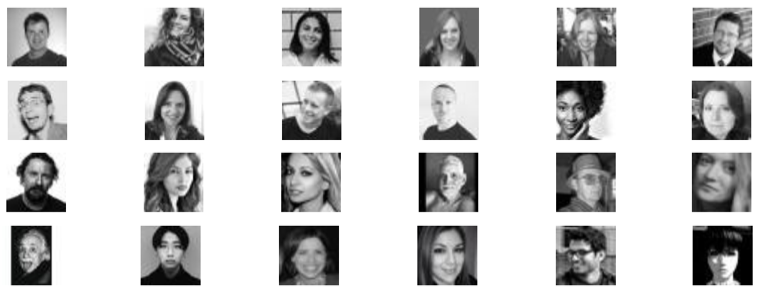
\includegraphics{assets/face.png}
\caption{``Faces at 40x40px''}
\end{figure}

If you zoom in on the faces, we're looking at 1600 individual pixels.
When dealing with grayscale images, a strategy can be assigning a value
of lightness on the scale of 0 to 1 to each of the 1,600 columns, with 0
being ``full white'' and 1 being ``full black'', and depending on the
saturity or lightness of each pixel - assign them a value in between.

\begin{figure}
\centering
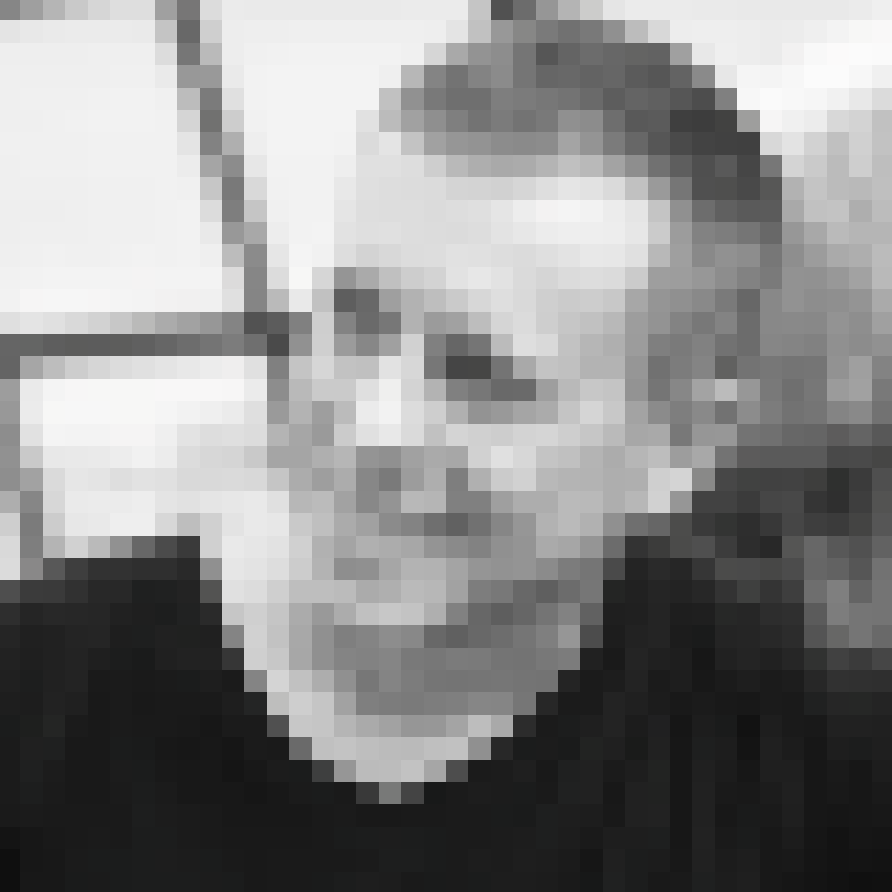
\includegraphics{assets/face1.png}
\caption{``Faces at 40x40px''}
\end{figure}

There are numerous good papers and resources that deal with the topic of
PCA use in image compression, such as the one by researchers as
Institute of Chemical Technology, Prague\footnote{\href{https://pdfs.semanticscholar.org/76a7/fc9d87736c8383576865cf50403e53e74848.pdf}{Principal
  Component Analysis in Image Processing}}, the one by Czech Institute
of Informatics, Robotics and Cybernetics\footnote{\href{http://people.ciirc.cvut.cz/~hlavac/TeachPresEn/11ImageProc/15PCA.pdf}{Principal
  Component Analysis (PCA) Application to images}}, and this one
here\footnote{\href{https://ece.gmu.edu/~hayes/courses/MachineLearning/Projects/Presentations/Norko.pdf}{Simple
  Image Classification using Principal Component Analysis (PCA)}}. By
the end of this PCA section, we'll also apply PCA on human faces to see
how image compression works in practice.

A 40x40 image is probably not interesting. If you're building an image
classifier using photos from an iPhone 7 plus, that's a resolution of
1,920 x 1,080 pixels (more than 2 million dimensions). And that's for a
single observation. Recall from your Practical Statistics course that a
way we can measure ``information'' is through variance, so a
dimensionality reduction method is essentially concerned with
representing as much ``variance'' as possible in as few dimensions as
possible.

The outcome of this transformation is that our original data (a matrix
\(X\)) is represented by a linearly transformed matrix, \(Z\), where
\(Z\) is typically a matrix with a lot fewer dimensions (commonly
\textless{}10) than \(X\). The first column of \(Z\) explains most of
the variance within \(X\), and the second explains a smaller amount of
variance than the first, and so on until the last column.

The objective of PCA is to find \(Q\), so that such a linear
transformation is possible.

If you remember the lessons from last week (Classification 2), I
demonstrated the use of \texttt{nearZeroVar} and \textbf{shown that
while eliminate \textasciitilde{}50\% of the original predictors we
still retain enough information} to build a multi-class classifier that
has a 99.98\% out-of-box accuracy. The features that were eliminated are
redundant in that they add little value or that they may just represent
``noise''. PCA shares the same objective, but does it differently: it
looks for correlation within our data and use that redundancy to create
a new matrix \(Z\) with just enough dimensions to explain most of the
variance in the original data. The new variables of matrix \(Z\) are
called \textbf{principal components}.

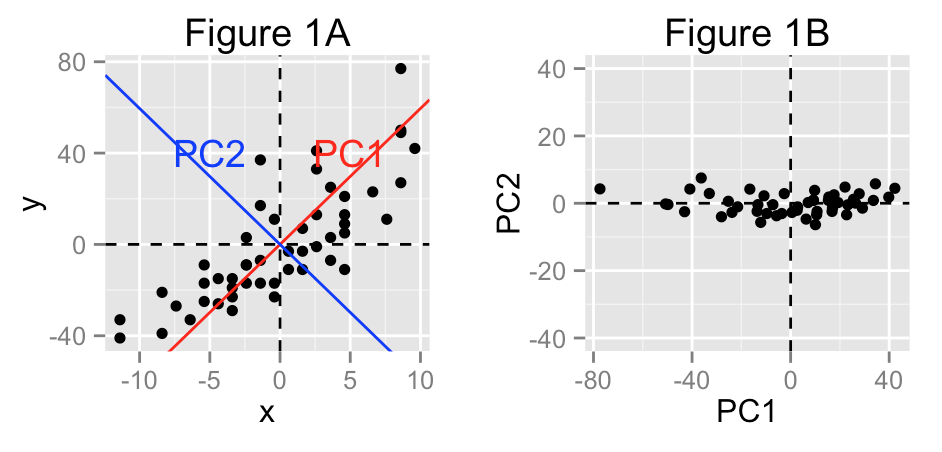
\includegraphics{assets/pca1.png} If you look at Figure 1A, our original
data sits on a plane with \texttt{x}and \texttt{y} coordinates. Two
dimensions (x and y, respectively) are required in Figure 1A to describe
the variance in our data fully.

However, supposed we identify two other axes to describe the same data,
and one of them is directly orthogonal to the other one: we can now
measure the variance in our data using just these axes (we call them
\textbf{principal components}). We identify the PC1 axis as the first
principal component because using only one principal component, this
would be the one that explain the most amount of variation. The PC2 axis
is then selected, again with the objective of explaining the most amount
of variation.

If we hold PC2 as constant (say, 0) then we reduce the dimensions from
two to only one, which is by projecting each data point onto PC1. We do
lose some variation as our observations are not exactly 0 on the PC2
axis, but since they are very close to being 0, the variation we lose
from reducing one dimension is a tradeoff we want to accept.

(Recall our lessons from Regression Model, when I introduce \texttt{VIF}
to show how if variable ``Police Expenditure this year'' can be
sufficiently explained by variable ``Police Expenditure last year'' then
we don't need both variables)

Other applications of PCA:\\
- Pattern discovery on high dimensional data\\
- Identify variables that are highly correlated with others\\
- Visualizing high dimensional data

\textbf{Dive Deeper:} Which of the two following data set are going to
be helped most by Principal Component Analysis (PCA)?

\begin{Shaded}
\begin{Highlighting}[]
\KeywordTok{set.seed}\NormalTok{(}\DecValTok{100}\NormalTok{)}
\KeywordTok{par}\NormalTok{(}\DataTypeTok{mfrow=}\KeywordTok{c}\NormalTok{(}\DecValTok{1}\NormalTok{,}\DecValTok{2}\NormalTok{))}
\NormalTok{x <-}\StringTok{ }\KeywordTok{runif}\NormalTok{(}\DecValTok{100}\NormalTok{)}
\KeywordTok{plot}\NormalTok{(}\DataTypeTok{x=}\NormalTok{x, }\DataTypeTok{y=}\KeywordTok{runif}\NormalTok{(}\DecValTok{100}\NormalTok{), }\DataTypeTok{pch=}\DecValTok{19}\NormalTok{, }\DataTypeTok{cex=}\FloatTok{0.5}\NormalTok{, }\DataTypeTok{xlim=}\KeywordTok{c}\NormalTok{(}\OperatorTok{-}\FloatTok{0.5}\NormalTok{, }\FloatTok{1.5}\NormalTok{), }\DataTypeTok{ylim=}\KeywordTok{c}\NormalTok{(}\OperatorTok{-}\FloatTok{0.5}\NormalTok{, }\FloatTok{1.5}\NormalTok{), }\DataTypeTok{main=}\StringTok{"Blind Tasting"}\NormalTok{, }\DataTypeTok{xlab=}\StringTok{"wine age"}\NormalTok{, }\DataTypeTok{ylab=}\StringTok{"score"}\NormalTok{)}
\KeywordTok{plot}\NormalTok{(}\DataTypeTok{x=}\NormalTok{x, }\DataTypeTok{y=}\NormalTok{x}\OperatorTok{+}\KeywordTok{runif}\NormalTok{(}\DecValTok{100}\NormalTok{, }\FloatTok{-0.1}\NormalTok{, }\FloatTok{0.1}\NormalTok{), }\DataTypeTok{pch=}\DecValTok{19}\NormalTok{, }\DataTypeTok{cex=}\FloatTok{0.5}\NormalTok{, }\DataTypeTok{xlim=}\KeywordTok{c}\NormalTok{(}\OperatorTok{-}\FloatTok{0.5}\NormalTok{, }\FloatTok{1.5}\NormalTok{), }\DataTypeTok{ylim=}\KeywordTok{c}\NormalTok{(}\OperatorTok{-}\FloatTok{0.5}\NormalTok{, }\FloatTok{1.5}\NormalTok{), }\DataTypeTok{main=}\StringTok{"Logistic Machinery"}\NormalTok{, }\DataTypeTok{xlab=}\StringTok{"temperature"}\NormalTok{, }\DataTypeTok{ylab=}\StringTok{"pressure"}\NormalTok{)}
\end{Highlighting}
\end{Shaded}

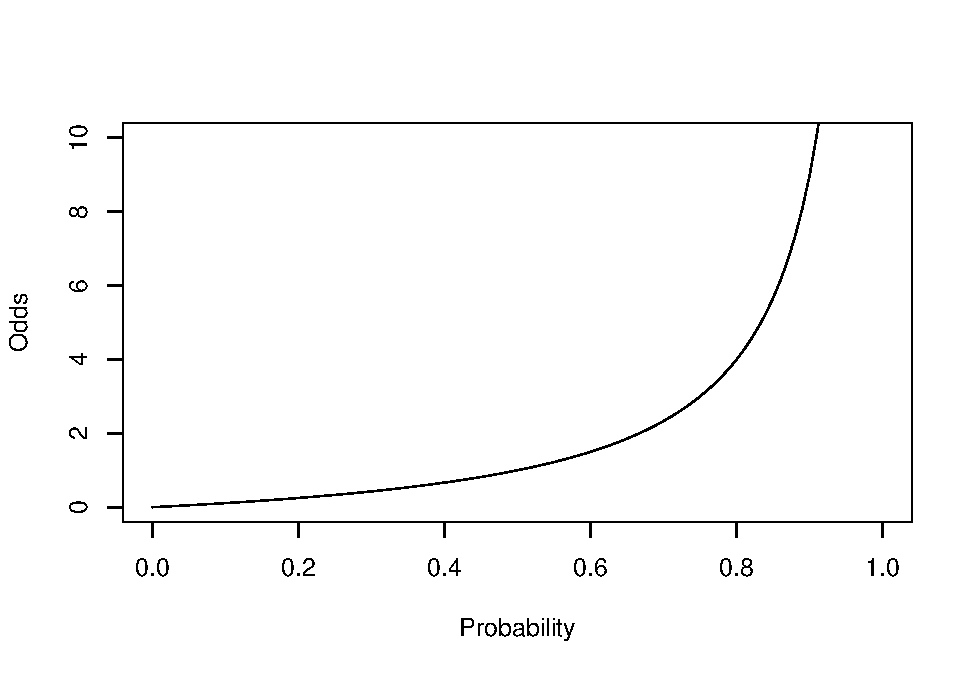
\includegraphics{unsupervised_files/figure-latex/unnamed-chunk-2-1.pdf}

\hypertarget{step-by-step-pca-analysis-on-property-sales-in-nyc}{%
\subsection{Step-by-step: PCA Analysis on Property Sales in
NYC}\label{step-by-step-pca-analysis-on-property-sales-in-nyc}}

Let's start by reading in a dataset which is concatenated\footnote{\href{https://www.kaggle.com/new-york-city/nyc-property-sales}{City
  of New York, NYC Property Sales}} from the New York City Department of
Finance and mada available by City of New York. This dataset is a record
of every building or building unit (apartment, etc.) sold in the New
York City property market over a 12-month period:

\begin{Shaded}
\begin{Highlighting}[]
\NormalTok{property <-}\StringTok{ }\KeywordTok{read.csv}\NormalTok{(}\StringTok{"data_input/nyc.csv"}\NormalTok{)}
\end{Highlighting}
\end{Shaded}

\texttt{BOROUGH}: A digit code for the borough the property is located
in; in order these are Manhattan (1), Bronx (2), Brooklyn (3), Queens
(4), and Staten Island (5)\\
\texttt{NEIGHBORHOOD}: The neighborhood name\\
\texttt{BUILDING.CLASS.CATEGORY}: Category class of the
property\footnote{\href{http://www1.nyc.gov/assets/finance/jump/hlpbldgcode.html}{City
  of New York, Building Classification}}\\
\texttt{TAX.CLASS.AT.PRESENT}, \texttt{TAX.CLASS.AT.TIME.OF.SALE}:
\texttt{BLOCK}, \texttt{LOT}: The combination of borough, block, and lot
forms a unique key for property in New York City\\
\texttt{EASE.MENT}:An easement is a right, such as a right of way, which
allows an entity to make limited use of another's real property\\
\texttt{BUILDING.CLASS.AT.PRESENT},
\texttt{BUILDING.CLASS.AT.TIME.OF.SALE}: The type of building at various
points in time, (for example ``A''" signifies one-family homes, ``O''
signifies office buildings. ``R'' signifies condominiums)\footnote{\href{http://www1.nyc.gov/assets/finance/jump/hlpbldgcode.html}{City
  of New York, Building Classification}}\\
\texttt{ADDRESS}: Street address of the property\\
\texttt{APARTMENT.NUMBER}: Apartment number if applicable\\
\texttt{ZIP.CODE}: The property's postal code\\
\texttt{RESIDENTIAL.UNTIS}: The number of residential units at the
listed property\\
\texttt{COMMERCIAL.UNITS}: The number of commercial units at the listed
property\\
\texttt{LAND.SQUARE.FEET}: The land area of the property listed in
square feet\\
\texttt{GROSS.SQUARE.FEET}: The total area of all the floors of a
building as measured from the exterior surfaces of the outside walls of
the building, including the land area and space within any building or
structure on the property\\
\texttt{YEAR.BUILT}: Year the property was built\\
\texttt{SALE.PRICE}: Price paid for the property\\
\texttt{SALE.DATE}: Date the property sold

Many of these property is sold with a nonsensically small dollar amount,
commonly \$0. These sales actually represent a transfer of ownership
without a cash consideration - such as when parents transfer ownership
to a child\footnote{\href{http://www1.nyc.gov/assets/finance/downloads/pdf/07pdf/glossary_rsf071607.pdf}{City
  of New York, Glossary of Terms for Property Sales Files}}.

This dataset uses the financial definition of a building/building unit,
for tax purposes. In case a single entity owns the building in question,
a sale covers the value of the entire building. In case a building is
owned piecemeal by its residents (a condominium), a sale refers to a
single apartment (or group of apartments) owned by some individual.

I'm going to do some cleaning and pre-processing using \texttt{dplyr},
and have the final dataset stored in a variable named \texttt{ppt}:

\begin{Shaded}
\begin{Highlighting}[]
\NormalTok{ppt <-}\StringTok{ }\NormalTok{property }\OperatorTok\StringTok{ }
\StringTok{  }\KeywordTok{mutate}\NormalTok{(}\DataTypeTok{LAND.SQUARE.FEET =} \KeywordTok{as.integer}\NormalTok{(LAND.SQUARE.FEET),}
         \DataTypeTok{GROSS.SQUARE.FEET =} \KeywordTok{as.integer}\NormalTok{(GROSS.SQUARE.FEET),}
         \DataTypeTok{SALE.PRICE =} \KeywordTok{as.integer}\NormalTok{(SALE.PRICE)}
\NormalTok{         ) }\OperatorTok\StringTok{ }
\StringTok{  }\KeywordTok{select_if}\NormalTok{(is.integer) }\OperatorTok\StringTok{ }
\StringTok{  }\KeywordTok{select}\NormalTok{(}\OperatorTok{!}\KeywordTok{c}\NormalTok{(X, BOROUGH, BLOCK, LOT, ZIP.CODE)) }\OperatorTok\StringTok{ }
\StringTok{  }\KeywordTok{filter}\NormalTok{(}\KeywordTok{complete.cases}\NormalTok{(.))}

\KeywordTok{str}\NormalTok{(ppt)}
\end{Highlighting}
\end{Shaded}

\begin{verbatim}
## 'data.frame':    48243 obs. of  8 variables:
##  $ RESIDENTIAL.UNITS        : int  5 10 6 8 24 10 24 3 4 5 ...
##  $ COMMERCIAL.UNITS         : int  0 0 0 0 0 0 0 1 1 1 ...
##  $ TOTAL.UNITS              : int  5 10 6 8 24 10 24 4 5 6 ...
##  $ LAND.SQUARE.FEET         : int  1633 2272 2369 1750 4489 3717 4131 1520 2201 1779 ...
##  $ GROSS.SQUARE.FEET        : int  6440 6794 4615 4226 18523 12350 16776 3360 5608 3713 ...
##  $ YEAR.BUILT               : int  1900 1913 1900 1920 1920 2009 1928 1910 1900 1910 ...
##  $ TAX.CLASS.AT.TIME.OF.SALE: int  2 2 2 2 2 2 2 2 2 2 ...
##  $ SALE.PRICE               : int  6625000 3936272 8000000 3192840 16232000 10350000 11900000 3300000 7215000 4750000 ...
\end{verbatim}

We've established earlier that correlations in the data makes some
variables redundant. In our regression models class, we observe that if
we can predict ``police expenditure this year'' accurately from ``police
expenditure last year'', then one of these variables is redundant.
Post-PCA, the matrix \(Z\) should be one where every dimension is
uncorrelated.

\textbf{Discussion:} Which of the following plot shows variables that
are uncorrelated?

\begin{Shaded}
\begin{Highlighting}[]
\KeywordTok{set.seed}\NormalTok{(}\DecValTok{100}\NormalTok{)}
\KeywordTok{par}\NormalTok{(}\DataTypeTok{mfrow=}\KeywordTok{c}\NormalTok{(}\DecValTok{1}\NormalTok{,}\DecValTok{3}\NormalTok{))}
\NormalTok{x <-}\StringTok{ }\KeywordTok{runif}\NormalTok{(}\DecValTok{100}\NormalTok{)}
\KeywordTok{plot}\NormalTok{(}\DataTypeTok{x=}\NormalTok{x, }\DataTypeTok{y=}\OperatorTok{-}\NormalTok{x}\OperatorTok{+}\KeywordTok{runif}\NormalTok{(}\DecValTok{100}\NormalTok{, }\DecValTok{1}\NormalTok{, }\FloatTok{1.2}\NormalTok{), }\DataTypeTok{pch=}\DecValTok{19}\NormalTok{, }\DataTypeTok{cex=}\FloatTok{0.5}\NormalTok{, }\DataTypeTok{xlim=}\KeywordTok{c}\NormalTok{(}\OperatorTok{-}\FloatTok{0.5}\NormalTok{, }\FloatTok{1.5}\NormalTok{), }\DataTypeTok{ylim=}\KeywordTok{c}\NormalTok{(}\OperatorTok{-}\FloatTok{0.5}\NormalTok{, }\FloatTok{1.5}\NormalTok{), }\DataTypeTok{main=}\StringTok{"Sale Price of Vehicles"}\NormalTok{, }\DataTypeTok{xlab=}\StringTok{"Age"}\NormalTok{, }\DataTypeTok{ylab=}\StringTok{"Sale Price"}\NormalTok{)}

\KeywordTok{plot}\NormalTok{(}\DataTypeTok{x=}\NormalTok{x, }\DataTypeTok{y=}\KeywordTok{runif}\NormalTok{(}\DecValTok{100}\NormalTok{), }\DataTypeTok{pch=}\DecValTok{19}\NormalTok{, }\DataTypeTok{cex=}\FloatTok{0.5}\NormalTok{, }\DataTypeTok{xlim=}\KeywordTok{c}\NormalTok{(}\OperatorTok{-}\FloatTok{0.5}\NormalTok{, }\FloatTok{1.5}\NormalTok{), }\DataTypeTok{ylim=}\KeywordTok{c}\NormalTok{(}\OperatorTok{-}\FloatTok{0.5}\NormalTok{, }\FloatTok{1.5}\NormalTok{), }\DataTypeTok{main=}\StringTok{"Blind Tasting"}\NormalTok{, }\DataTypeTok{xlab=}\StringTok{"wine age"}\NormalTok{, }\DataTypeTok{ylab=}\StringTok{"score"}\NormalTok{)}

\KeywordTok{plot}\NormalTok{(}\DataTypeTok{x=}\NormalTok{x, }\DataTypeTok{y=}\NormalTok{x}\OperatorTok{+}\KeywordTok{runif}\NormalTok{(}\DecValTok{100}\NormalTok{, }\FloatTok{-0.1}\NormalTok{, }\FloatTok{0.1}\NormalTok{), }\DataTypeTok{pch=}\DecValTok{19}\NormalTok{, }\DataTypeTok{cex=}\FloatTok{0.5}\NormalTok{, }\DataTypeTok{xlim=}\KeywordTok{c}\NormalTok{(}\OperatorTok{-}\FloatTok{0.5}\NormalTok{, }\FloatTok{1.5}\NormalTok{), }\DataTypeTok{ylim=}\KeywordTok{c}\NormalTok{(}\OperatorTok{-}\FloatTok{0.5}\NormalTok{, }\FloatTok{1.5}\NormalTok{), }\DataTypeTok{main=}\StringTok{"Logistic Machinery"}\NormalTok{, }\DataTypeTok{xlab=}\StringTok{"temperature"}\NormalTok{, }\DataTypeTok{ylab=}\StringTok{"pressure"}\NormalTok{)}
\end{Highlighting}
\end{Shaded}

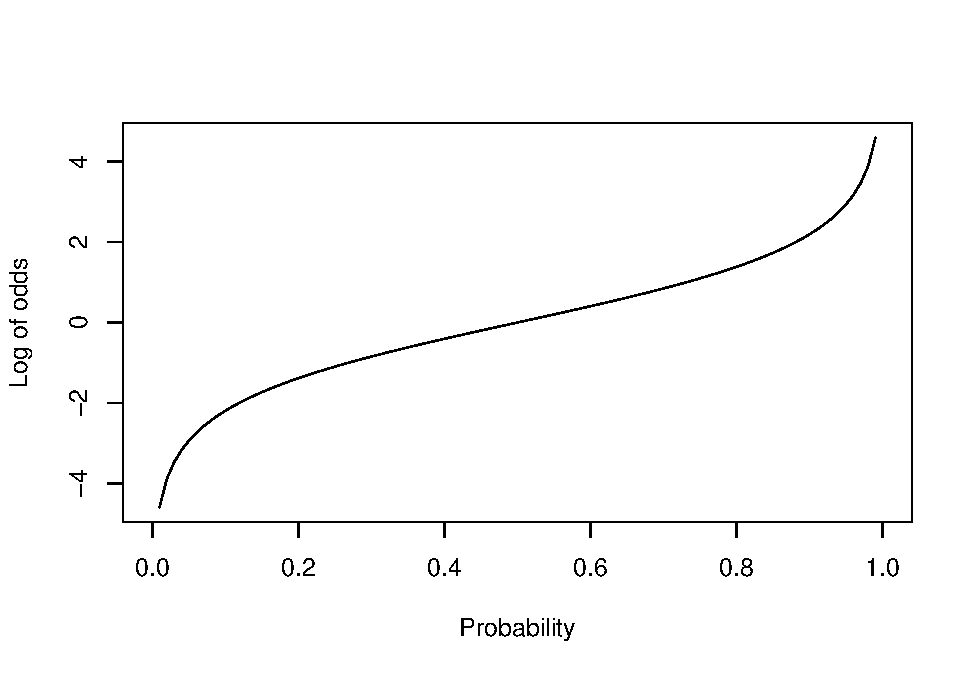
\includegraphics{unsupervised_files/figure-latex/unnamed-chunk-5-1.pdf}

The variables Age and Price in \texttt{Sale\ Price\ of\ Vehicle} are not
uncorrelated. If you plot a regression line on it, that line exhbits a
downward slope, and the correlation between Age and Sales Price would be
a value close to -1.

The variables Temperature and Pressure in \texttt{Logistic\ Machinery}
are also not uncorrelated. If you plot a regression line on it, that
line exhbit an upward slope, and the correlation between Temperature and
Pressure would be a value close to 1.

Intuitively, we conclude that the variables ``Blind Tasting'' are
uncorrelated because knowing the value of x does not give us any
indication of what the value of y may be.

Now if we follow the example in \textbf{pca1.png} (from the Principle
and Motivation) section and pick a new axis combination for
\texttt{Logistic\ Machinery} (which is the purple line labelled
\texttt{v1} and \texttt{v2} in the following picture), then the
distributions for temperature and pressure becomes uncorrelated under
the two new axes:

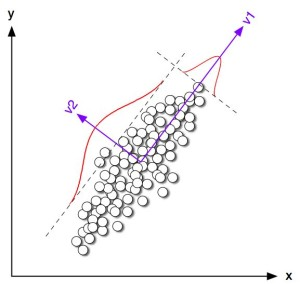
\includegraphics{assets/pca2.jpg}

\hypertarget{optional-eigenvalues-and-eigenvectors}{%
\subsubsection{{[}Optional{]} Eigenvalues and
Eigenvectors}\label{optional-eigenvalues-and-eigenvectors}}

If you have limited exposure to Matrix Algebra - feel free to skip this
sub-section. Concepts presented under this sub-section will not be
graded; In fact, R has really convenient built-in functions that help
you compute eigenvectors and eigenvalues so the inner-working is for the
most part optional for any practitioner.

In linear algebra and matrix theory, we learn that a vector when
multiplied by a matrix, changes its direction. When we take a
vector(2,3) and multiply it by a scale, say 2, then the resulting vector
would be (4,6) - the scalar scales the vector by a magnitude of 2.

Now if we take the same vector and multiply it by a matrix, the vector
being acted on changes direction: \$\$\left(

\begin{array}{cc} 
11\\
16
\end{array}

\right) = \left(

\begin{array}{cc} 
1 & 3\\
2 & 4
\end{array}

\right)

\left(

\begin{array}{cc} 
2\\ 
3 
\end{array}

\right)\$\$ In R, we use \texttt{\%*\%} to denote a matrix
multiplication:

\begin{Shaded}
\begin{Highlighting}[]
\KeywordTok{matrix}\NormalTok{(}\DecValTok{1}\OperatorTok{:}\DecValTok{4}\NormalTok{, }\DataTypeTok{nrow=}\DecValTok{2}\NormalTok{) }\OperatorTok\StringTok{ }\KeywordTok{as.vector}\NormalTok{(}\KeywordTok{c}\NormalTok{(}\DecValTok{2}\NormalTok{,}\DecValTok{3}\NormalTok{))}
\end{Highlighting}
\end{Shaded}

\begin{verbatim}
##      [,1]
## [1,]   11
## [2,]   16
\end{verbatim}

In a sense, we can think of the above operation as a matrix transforming
a vector into another vector: the resulting vector will (generally) have
a different direction and length than the original vector. There are
however a few notable exception to this:

\begin{itemize}
\tightlist
\item
  The matrix that acts on a vector without actually changing it at all
  is called the \textbf{identity matrix}. An identity matrix is a square
  matrix in which all the elements of the principal diagonal are ones
  and all other elements are zeros.
\end{itemize}

The (2,3) matrix multiplied by an identity matrix of size 2 is going to
result as a (2,3); neither the direction or the magnitude is changed.

\begin{Shaded}
\begin{Highlighting}[]
\KeywordTok{c}\NormalTok{(}\DecValTok{2}\NormalTok{,}\DecValTok{3}\NormalTok{) }\OperatorTok\StringTok{ }\KeywordTok{diag}\NormalTok{(}\DataTypeTok{nrow=}\DecValTok{2}\NormalTok{,}\DataTypeTok{ncol=}\DecValTok{2}\NormalTok{)}
\end{Highlighting}
\end{Shaded}

\begin{verbatim}
##      [,1] [,2]
## [1,]    2    3
\end{verbatim}

\begin{itemize}
\tightlist
\item
  The matrix that rotates every vector through a fixed angle is called a
  \textbf{rotation matrix}. The direction of a vector changes, but not
  its magnitude. Take the matrix, A, below and multiply it with (-3, 2)
  to get (3, -2). If you draw the two vectors you'll notice that they
  are of the same length with the second vector rotated at 180 degree to
  the first. Multiply A with (-20, 18) and the vector gets transformed
  to (20, -18), again rotated by 180 degree. As it turns out A is a
  rotation matrix that will transform a vector by 180 degree but without
  changing the magnitude of the vector. \[
  \left(\begin{array}{cc} 
  -1 & 0\\ 
  0 & -1 
  \end{array}\right)
  \left(\begin{array}{cc} 
  -3\\ 
  2
  \end{array}\right)
  \]
\end{itemize}

\begin{Shaded}
\begin{Highlighting}[]
\KeywordTok{matrix}\NormalTok{(}\KeywordTok{c}\NormalTok{(}\OperatorTok{-}\DecValTok{1}\NormalTok{,}\DecValTok{0}\NormalTok{,}\DecValTok{0}\NormalTok{,}\OperatorTok{-}\DecValTok{1}\NormalTok{),}\DecValTok{2}\NormalTok{,}\DecValTok{2}\NormalTok{) }\OperatorTok\StringTok{ }\KeywordTok{c}\NormalTok{(}\OperatorTok{-}\DecValTok{3}\NormalTok{,}\DecValTok{2}\NormalTok{)}
\end{Highlighting}
\end{Shaded}

\begin{verbatim}
##      [,1]
## [1,]    3
## [2,]   -2
\end{verbatim}

\includegraphics{assets/rotation.gif}

\begin{itemize}
\tightlist
\item
  For most matrices there are certain vectors, called
  \textbf{eigenvectors} whose directions don't change (except when it's
  scaled by -1, in which case its direction reversed) when acted on by
  the matrix. The effect on multiplying that matrix by such a vector,
  its eigenvector, is the same as multiplying the vector by a scalar.
  This scalar is a constant and is formally referred to as an
  \textbf{eigenvalue}. WHen we multiply matrix A by an eigenvector x,
  the result would be a constant \(\lambda\) multiply by x. The equation
  is hence:
\end{itemize}

\(Ax = \lambda x\), where the number \(\lambda\) is an eigenvalue of A.

\[
\left(\begin{array}{cc} 
2 & 3\\ 
2 & 1 
\end{array}\right)
\left(\begin{array}{cc} 
3\\ 
2
\end{array}\right)
=
\left(\begin{array}{cc} 
12\\ 
8
\end{array}\right)
=4
\left(\begin{array}{cc} 
3\\ 
2
\end{array}\right)
\\
2\left(\begin{array}{cc} 
3\\ 
2
\end{array}\right) = \left(\begin{array}{cc} 
6\\ 
4
\end{array}\right) \\
\left(\begin{array}{cc} 
2 & 3\\ 
2 & 1 
\end{array}\right)
\left(\begin{array}{cc} 
6\\ 
4
\end{array}\right)
=\left(\begin{array}{cc} 
24\\ 
16
\end{array}\right)
=4
\left(\begin{array}{cc} 
6\\ 
4
\end{array}\right)
\] Observe how a scaled eigenvector is still an eigenvector.

\hypertarget{intuition-and-practice-pca}{%
\subsubsection{Intuition and Practice:
PCA}\label{intuition-and-practice-pca}}

Remember earlier I mention that intuitively, the objective of a PCA is
to select new axis (new dimensions) for our plot and that these new
dimensions of our data are called \textbf{principal components}? The new
dimensions should have no correlation to each other (in the context of
dimensionality, correlation leads to redundancy!). If we have a
covariance matrix:

\begin{Shaded}
\begin{Highlighting}[]
\NormalTok{A <-}\StringTok{ }\KeywordTok{matrix}\NormalTok{(}\KeywordTok{c}\NormalTok{(}\FloatTok{1.04}\NormalTok{, }\FloatTok{0.77}\NormalTok{, }\FloatTok{0.77}\NormalTok{, }\FloatTok{0.68}\NormalTok{), }\DataTypeTok{nrow=}\DecValTok{2}\NormalTok{)}
\NormalTok{A}
\end{Highlighting}
\end{Shaded}

\begin{verbatim}
##      [,1] [,2]
## [1,] 1.04 0.77
## [2,] 0.77 0.68
\end{verbatim}

Recall from our Practical Statistics workshops that this means the
variance of our first variable is 1.04, the variance of the second
variable is 0.68 and the covariance between these two is 0.77.

Now \texttt{A} is a square symmetrical matrix, so it can be diagonalized
by choosing a new coordinate system given by its eigenvectors, the
corresponding eigenvalues will then replace the values on the diagonal.
Using this new coordinate system, our covariance matrix A will look
like:

\begin{Shaded}
\begin{Highlighting}[]
\KeywordTok{round}\NormalTok{(}\KeywordTok{matrix}\NormalTok{(}\KeywordTok{c}\NormalTok{(}\KeywordTok{eigen}\NormalTok{(A)}\OperatorTok{$}\NormalTok{values[}\DecValTok{1}\NormalTok{], }\DecValTok{0}\NormalTok{, }\DecValTok{0}\NormalTok{, }\KeywordTok{eigen}\NormalTok{(A)}\OperatorTok{$}\NormalTok{values[}\DecValTok{2}\NormalTok{]), }\DataTypeTok{nrow=}\DecValTok{2}\NormalTok{),}\DecValTok{2}\NormalTok{)}
\end{Highlighting}
\end{Shaded}

\begin{verbatim}
##      [,1] [,2]
## [1,] 1.65 0.00
## [2,] 0.00 0.07
\end{verbatim}

Now observe that with this transformation, the correlation between the
two variables is now zero. The maximum variance of 1.65 can be achieved
if we would take the projection on the first coordinate axis (reducing
the second axis), so it makes sense that the direction of the first
\textbf{principal component} is thus selected from the first eigenvector
of the covariance matrix.

Let's see one more example, and this time we'll make this more visual to
strengthen the intuition:

\begin{Shaded}
\begin{Highlighting}[]
\KeywordTok{set.seed}\NormalTok{(}\DecValTok{100}\NormalTok{)}
\NormalTok{x <-}\StringTok{ }\KeywordTok{runif}\NormalTok{(}\DecValTok{200}\NormalTok{)}
\NormalTok{A <-}\StringTok{ }\KeywordTok{data.frame}\NormalTok{(}\DataTypeTok{x=}\NormalTok{x, }\DataTypeTok{y=}\OperatorTok{-}\NormalTok{x}\OperatorTok{+}\KeywordTok{runif}\NormalTok{(}\DecValTok{100}\NormalTok{, }\FloatTok{1.05}\NormalTok{, }\FloatTok{1.25}\NormalTok{))}
\NormalTok{A <-}\StringTok{ }\KeywordTok{scale}\NormalTok{(A, }\DataTypeTok{center =}\NormalTok{ T)}
\KeywordTok{plot}\NormalTok{(A, }\DataTypeTok{cex=}\FloatTok{0.4}\NormalTok{)}
\end{Highlighting}
\end{Shaded}

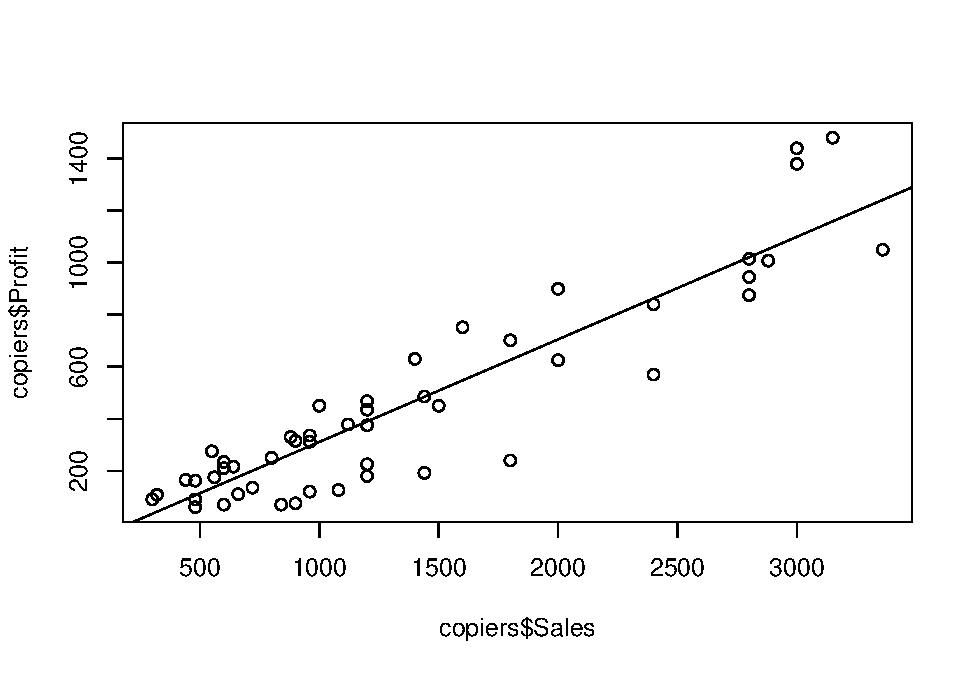
\includegraphics{unsupervised_files/figure-latex/unnamed-chunk-11-1.pdf}

Let's take a look at the covariance matrix of A:

\begin{Shaded}
\begin{Highlighting}[]
\KeywordTok{cov}\NormalTok{(A)}
\end{Highlighting}
\end{Shaded}

\begin{verbatim}
##           x         y
## x  1.000000 -0.982719
## y -0.982719  1.000000
\end{verbatim}

No surprised in the matrix above, as x and y are correlated with
themselves (hence 1), and that both of them are negatively (and
strongly) correlated. If we extract the first eigenvector and derive the
slope (we can think of this as principal component 1) and do the same
for the second eigenvector (principal component 2), we can then use
these two as the new coordinates for our plot later:

\begin{Shaded}
\begin{Highlighting}[]
\NormalTok{slope1 <-}\StringTok{ }\KeywordTok{eigen}\NormalTok{(}\KeywordTok{cov}\NormalTok{(A))}\OperatorTok{$}\NormalTok{vectors[}\DecValTok{1}\NormalTok{,}\DecValTok{1}\NormalTok{]}\OperatorTok{/}\KeywordTok{eigen}\NormalTok{(}\KeywordTok{cov}\NormalTok{(A))}\OperatorTok{$}\NormalTok{vectors[}\DecValTok{2}\NormalTok{,}\DecValTok{1}\NormalTok{]}
\NormalTok{slope2 <-}\StringTok{ }\KeywordTok{eigen}\NormalTok{(}\KeywordTok{cov}\NormalTok{(A))}\OperatorTok{$}\NormalTok{vectors[}\DecValTok{1}\NormalTok{,}\DecValTok{2}\NormalTok{]}\OperatorTok{/}\KeywordTok{eigen}\NormalTok{(}\KeywordTok{cov}\NormalTok{(A))}\OperatorTok{$}\NormalTok{vectors[}\DecValTok{2}\NormalTok{,}\DecValTok{2}\NormalTok{]}
\end{Highlighting}
\end{Shaded}

And now observe how we plot \texttt{slope1} and \texttt{slope2} onto the
original data. Take a second to observe that the two are orthogonal and
imagine remove the second axis (green), that would mean our observation
are projected onto a one-dimensional line (blue line) - we would lose
some information, but as it turns out, that blue line captures the most
amount of variation in our data and so that information loss from
removing the green line is the most minimal compared to other possible
combinations of axes / other possible combinations of coordinate system.

\begin{Shaded}
\begin{Highlighting}[]
\KeywordTok{par}\NormalTok{(}\DataTypeTok{mar=}\KeywordTok{c}\NormalTok{(}\DecValTok{1}\NormalTok{,}\DecValTok{1}\NormalTok{,}\DecValTok{1}\NormalTok{,}\DecValTok{1}\NormalTok{))}
\KeywordTok{plot}\NormalTok{(A, }\DataTypeTok{pch=}\DecValTok{19}\NormalTok{, }\DataTypeTok{cex=}\FloatTok{0.25}\NormalTok{, }\DataTypeTok{xlim=}\KeywordTok{c}\NormalTok{(}\OperatorTok{-}\FloatTok{1.5}\NormalTok{,}\FloatTok{1.5}\NormalTok{), }\DataTypeTok{ylim=}\KeywordTok{c}\NormalTok{(}\OperatorTok{-}\FloatTok{1.5}\NormalTok{,}\FloatTok{1.5}\NormalTok{))}
\KeywordTok{abline}\NormalTok{(}\DataTypeTok{h =} \DecValTok{0}\NormalTok{, }\DataTypeTok{lty=}\DecValTok{3}\NormalTok{, }\DataTypeTok{lwd=}\FloatTok{0.6}\NormalTok{)}
\KeywordTok{abline}\NormalTok{(}\DataTypeTok{v =} \DecValTok{0}\NormalTok{, }\DataTypeTok{lty=}\DecValTok{3}\NormalTok{, }\DataTypeTok{lwd=}\FloatTok{0.6}\NormalTok{)}
\KeywordTok{lines}\NormalTok{(A[,}\DecValTok{1}\NormalTok{], A[,}\DecValTok{1}\NormalTok{] }\OperatorTok{*}\StringTok{ }\NormalTok{slope1, }\DataTypeTok{col=}\StringTok{"blue"}\NormalTok{)}
\KeywordTok{lines}\NormalTok{(A[,}\DecValTok{1}\NormalTok{], A[,}\DecValTok{1}\NormalTok{] }\OperatorTok{*}\StringTok{ }\NormalTok{slope2, }\DataTypeTok{col=}\StringTok{"green"}\NormalTok{)}
\end{Highlighting}
\end{Shaded}

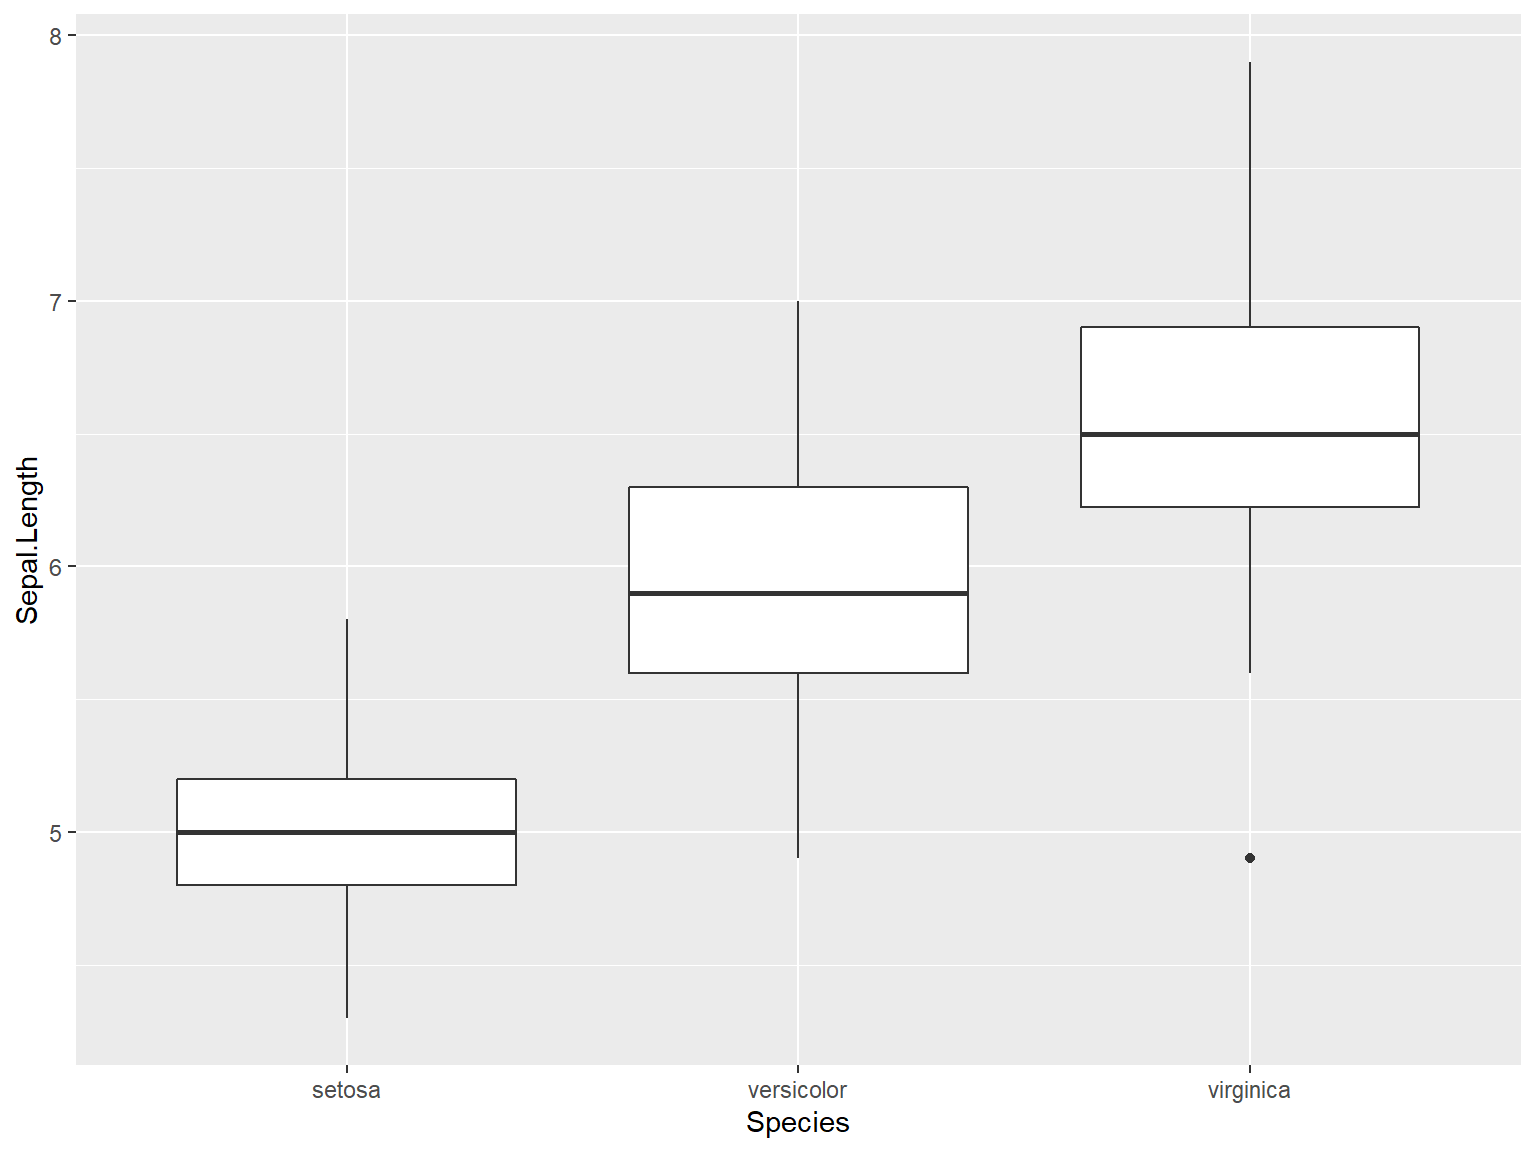
\includegraphics{unsupervised_files/figure-latex/unnamed-chunk-14-1.pdf}

\hypertarget{application-of-pca-dimensionality-reduction-on-nyc-property-sales}{%
\subsection{Application of PCA: Dimensionality Reduction on NYC Property
Sales}\label{application-of-pca-dimensionality-reduction-on-nyc-property-sales}}

With all the newly equipped knowledge, we'll now see how PCA is applied
to to our property sales dataset. First, let's take a look at the
covariance matrix of the \texttt{ppt} dataset. Realize that the
\texttt{ppt} matrix is not centered / scaled yet:

\begin{Shaded}
\begin{Highlighting}[]
\KeywordTok{cov}\NormalTok{(ppt)[}\DecValTok{1}\OperatorTok{:}\DecValTok{3}\NormalTok{,]}
\end{Highlighting}
\end{Shaded}

\begin{verbatim}
##                   RESIDENTIAL.UNITS COMMERCIAL.UNITS TOTAL.UNITS
## RESIDENTIAL.UNITS        305.049227         2.453481    307.4475
## COMMERCIAL.UNITS           2.453481       120.715187    123.1605
## TOTAL.UNITS              307.447502       123.160464    430.5673
##                   LAND.SQUARE.FEET GROSS.SQUARE.FEET YEAR.BUILT
## RESIDENTIAL.UNITS        220200.79         318448.58  220.67016
## COMMERCIAL.UNITS          18207.15          21369.67   27.67792
## TOTAL.UNITS              238340.88         339744.66  242.55301
##                   TAX.CLASS.AT.TIME.OF.SALE SALE.PRICE
## RESIDENTIAL.UNITS                 0.3452129   28836513
## COMMERCIAL.UNITS                  0.4873359    5362349
## TOTAL.UNITS                       0.8811511   34181340
\end{verbatim}

If we extract our principal components from the above matrix, the result
is not going to be useful. When we think of PCA as a variance maximizing
exercise, this become clearer: when we our PCA on the above data
(un-scaled), the amount of variance explained by the different principal
components is going to be dominated by variables that are on a larger
range.

\begin{Shaded}
\begin{Highlighting}[]
\KeywordTok{plot}\NormalTok{(}\KeywordTok{prcomp}\NormalTok{(ppt))}
\end{Highlighting}
\end{Shaded}

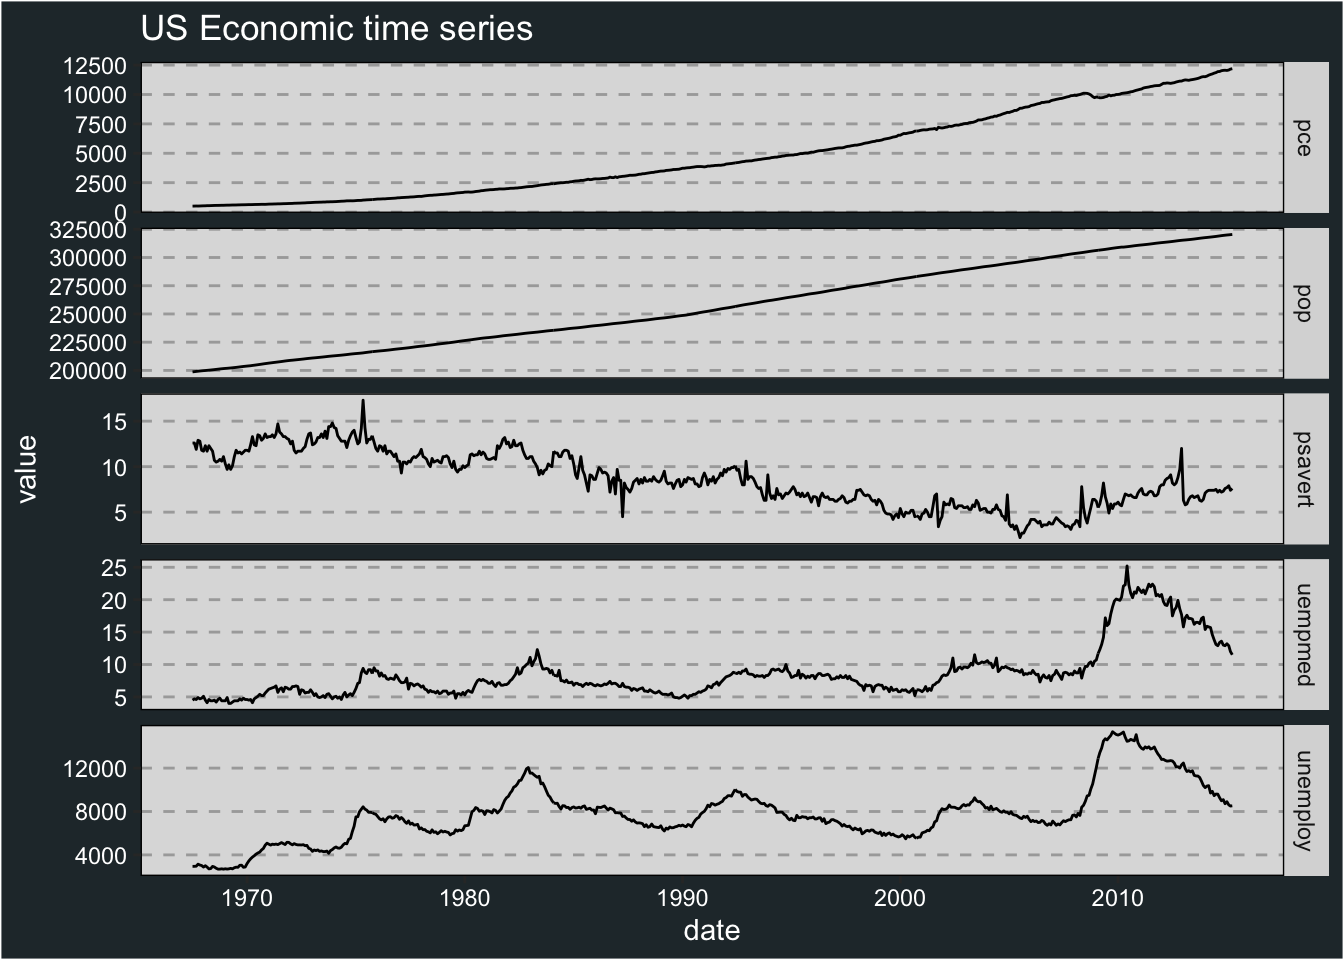
\includegraphics{unsupervised_files/figure-latex/unnamed-chunk-16-1.pdf}

If we had standardized the data first, and perform our principal
component analysis, we would get a much more sensible output:

\begin{Shaded}
\begin{Highlighting}[]
\NormalTok{ppt_z <-}\StringTok{ }\KeywordTok{scale}\NormalTok{(ppt, }\DataTypeTok{center =}\NormalTok{ T, }\DataTypeTok{scale=}\NormalTok{T)}
\KeywordTok{plot}\NormalTok{(}\KeywordTok{prcomp}\NormalTok{(ppt_z))}
\end{Highlighting}
\end{Shaded}

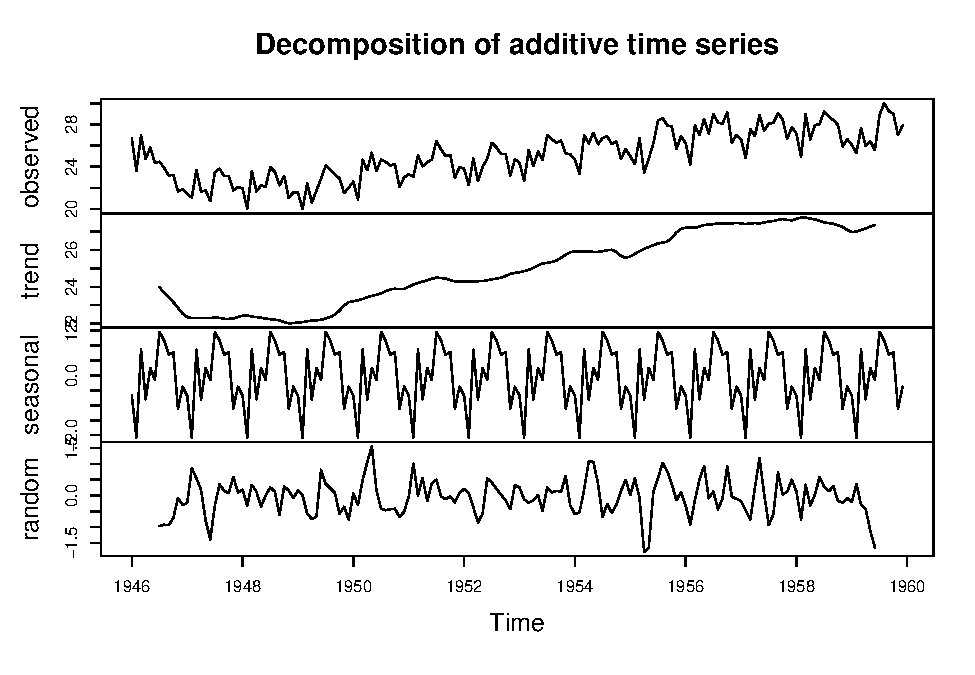
\includegraphics{unsupervised_files/figure-latex/unnamed-chunk-17-1.pdf}

\begin{Shaded}
\begin{Highlighting}[]
\CommentTok{# equivalent: plot(prcomp(ppt, scale=T))}
\end{Highlighting}
\end{Shaded}

This here gives us a clearer idea that the other components contributed
in retaining the variance within our data as well. So as a rule of
thumb: when we're looking for features to retain in a dimensionality
reduction exercise, make sure we scale or normalize our data before
running PCA.

Earlier we use the \texttt{prcomp()} function, if we want the data to be
centered around the mean, we can specify \texttt{center=TRUE} in our
function call; If we wanted the data to be scaled to have unit variance
before PCA takes place, we can add \texttt{scale=TRUE}. This is
generally advisable when our data has different units.

Look at the last plot a couple of lines above and pay special attention
to the \emph{equivalent code} commented out.

Let's learn another plot commonly used in PCA analysis, the
\texttt{biplot()}. A \texttt{biplot()} function expects a
\texttt{prcomp} object, renders the following:

\begin{Shaded}
\begin{Highlighting}[]
\NormalTok{ppt_small <-}\StringTok{ }\NormalTok{ppt[}\DecValTok{1}\OperatorTok{:}\DecValTok{100}\NormalTok{, ]}
\KeywordTok{biplot}\NormalTok{(}\KeywordTok{prcomp}\NormalTok{(ppt_small, }\DataTypeTok{scale=}\NormalTok{T), }\DataTypeTok{cex=}\FloatTok{0.5}\NormalTok{)}
\end{Highlighting}
\end{Shaded}

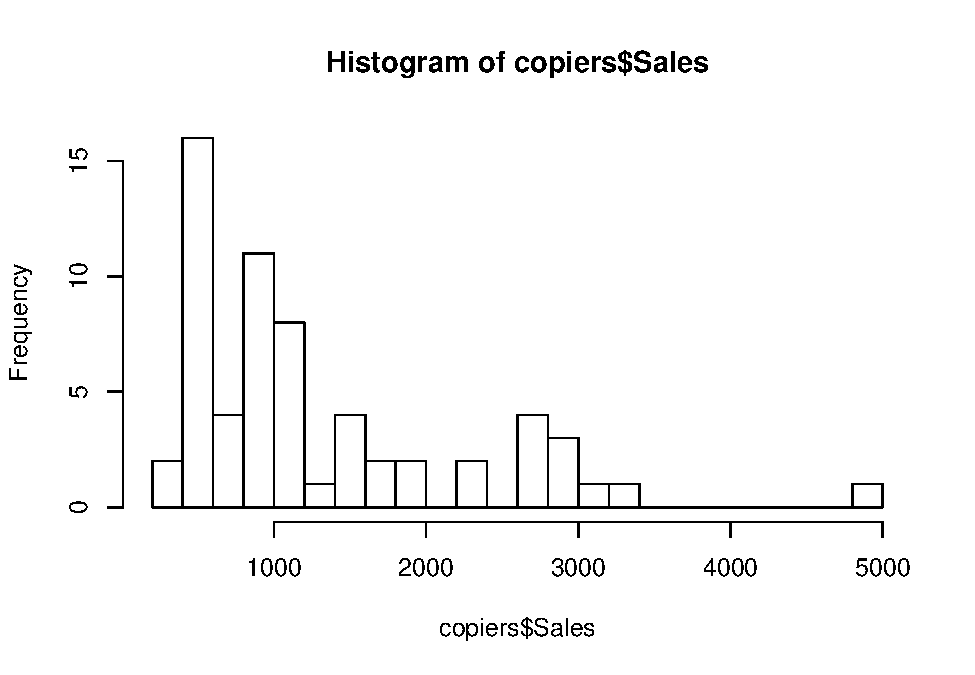
\includegraphics{unsupervised_files/figure-latex/unnamed-chunk-18-1.pdf}

The plot shows:\\
- Where the first 100 property sales within our data is positioned in
terms of PC1 and PC2, represented by text labels\\
- The loading of each variable on PC1 and PC2, represented by the red
arrow

The x and y axes are now replaced with PC1 and PC2, in that order. The
top and right axes indicate the loadings. In many cases, practitioners
can use only the first two principal components and still retain enough
``information'' within the data - the first two principal components, as
it turned out very often have retain most of the variance in our data
and so the reduced dimensionality can result in a visual representation
like the one above.

Since it is useful to ``visually'' represent the variability in our
observations (rows) and our variables (columns), we can make use of R's
built-in function, \texttt{biplot} to achieving that.

For example, if we're paying attention to the plot, we can see that most
of the property sales tend to be quite characteristically similar as
measured by PC1 and PC2 - that explains how most points are concentrated
in the ``top right'' corner. We also see that \texttt{GROSS.SQUARE.FEET}
and \texttt{LAND.SQUARE.FEET} are close to almost overlapping each
other, suggesting that these two variables are characteristically
similar and capture very identical information in the data. Observe also
that \texttt{RESIDENTIAL.UNITS} and \texttt{TOTAL.UNITS} are also very
close together in space, and both are variables that contribute strongly
to the second principal component.

\begin{Shaded}
\begin{Highlighting}[]
\KeywordTok{cor}\NormalTok{(ppt_small}\OperatorTok{$}\NormalTok{GROSS.SQUARE.FEET, ppt_small}\OperatorTok{$}\NormalTok{LAND.SQUARE.FEET)}
\end{Highlighting}
\end{Shaded}

\begin{verbatim}
## [1] 0.7452589
\end{verbatim}

\begin{Shaded}
\begin{Highlighting}[]
\KeywordTok{cor}\NormalTok{(ppt_small}\OperatorTok{$}\NormalTok{RESIDENTIAL.UNITS, ppt_small}\OperatorTok{$}\NormalTok{TOTAL.UNITS)}
\end{Highlighting}
\end{Shaded}

\begin{verbatim}
## [1] 0.9514941
\end{verbatim}

In addition to looking for observations and variables that have high
proximity in this new vector space, we can also look for ones that are
distant. We can observe a few outliers that are quite distinguished from
the others (property sales \#51, \#32 and \#96). We can inspect these
property sales by flagging them for a closer look later. The arrows
representing \texttt{RESIDENTIAL.UNITS} and the one representing
\texttt{COMMERCIAL.UNITS} are pointing in rather separate directions
(and magnitude), which means (really sketching the surface of intuition
here) that their contribution to each of the 2 principal components are
sufficiently differentiated.

Let's do one more practice. This time we'll plot the first 300 of those
property sales. Try and observe the plot - did you see any outlier?

\begin{Shaded}
\begin{Highlighting}[]
\NormalTok{ppt_small <-}\StringTok{ }\NormalTok{ppt[}\DecValTok{1}\OperatorTok{:}\DecValTok{300}\NormalTok{, ]}
\KeywordTok{biplot}\NormalTok{(}\KeywordTok{prcomp}\NormalTok{(ppt_small, }\DataTypeTok{scale=}\NormalTok{T), }\DataTypeTok{cex=}\FloatTok{0.5}\NormalTok{)}
\end{Highlighting}
\end{Shaded}

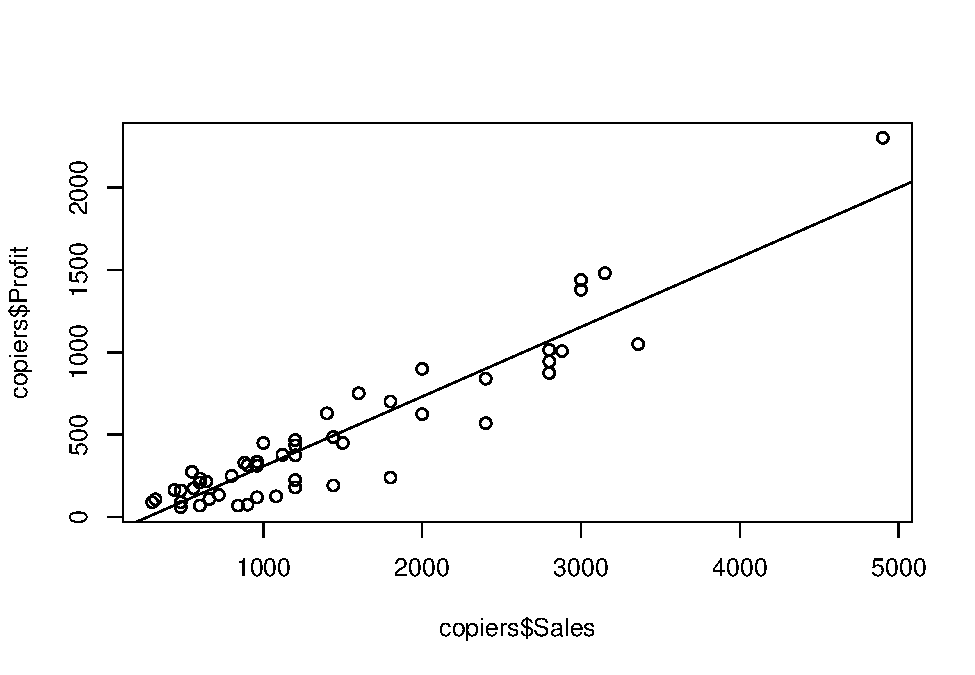
\includegraphics{unsupervised_files/figure-latex/unnamed-chunk-20-1.pdf}

We can further inspect some of these outliers (110, 114, 115, and 116
and 118). In real world applications, we would likely also have buyer
and seller information, and these 4 transactions (out of 300) may have
been singled out - say for tax auditing purposes, to see if there's foul
play or anything worthy of further, manual inspection.

As we inspect the 5 property sales below, pay close attention to the 5
ones we we identified above. Notice that in our biplot, we're really
only relying on two ``dimensions'' (as opposed to the original
dimensions in our dataset), PC1 and PC2 respectively, to ``summarize''
our data, and isn't it quite interesting that a 2-d plot is able to
capture most of the variation between observations \textbf{as well as}
between the original variables?

116 is the closest point to 118 in the biplot, and both turns out to be
among the most distant from the rest of our observations. If you look at
the raw data itself, that's immediately clear: both are property sales
involving only 1 commercial unit and yet commanding a very hefty price
tag, in some cases 5 times more expensive than another sale involving
529 residential units (in New York City!).

\begin{Shaded}
\begin{Highlighting}[]
\KeywordTok{as.matrix}\NormalTok{(ppt[}\DecValTok{105}\OperatorTok{:}\DecValTok{120}\NormalTok{,}\KeywordTok{c}\NormalTok{(}\DecValTok{1}\OperatorTok{:}\DecValTok{2}\NormalTok{,}\DecValTok{5}\OperatorTok{:}\DecValTok{6}\NormalTok{,}\DecValTok{8}\NormalTok{)])}
\end{Highlighting}
\end{Shaded}

\begin{verbatim}
##     RESIDENTIAL.UNITS COMMERCIAL.UNITS GROSS.SQUARE.FEET YEAR.BUILT SALE.PRICE
## 105                 0               12             55473       1926    1161500
## 106                 0               12             81375       1907    5000000
## 107                 0               15             79465       1913     220000
## 108                 0                1             81000       2007  105592700
## 109                 0                1            177000       2010  128177800
## 110               529                9            473391       1929  212500000
## 111                 0                1            122859       2008  139657500
## 112                 0                9             80185       1913   51000000
## 113                 0                2              4554       1930   16540319
## 114               476                6            400531       1929  239114603
## 115               317                6            303175       1921  182391612
## 116                 0                1            993569       1983  652000000
## 117                 0               23            566858       1973    3288000
## 118                 0                1           1617206       1987 1040000000
## 119                 0               52            527605       1912   54052917
## 120                 0                5             21520       1948   12500000
\end{verbatim}

110, 114, 115 are close to each other on the biplot and realize that in
the original data, they are similar to each other in that both involve a
high number of residential units (probably a condominium or large
apartment) and that all three are relatively old buildings - built
between the year 1921 and 1929. In practice, we would identify these
properties by a transaction id, and investigate further for any
interesting ``pattern'': if they are from the same property developer,
share a same sales agency etc. A biplot, using only two axis,
communicates hidden structure that are otherwise difficult to
meaningfully visualize or compare.

Let's go into the inner workings of the PCA by inspecting its summary:

\begin{Shaded}
\begin{Highlighting}[]
\NormalTok{ppt_prcomp <-}\StringTok{ }\KeywordTok{prcomp}\NormalTok{(ppt_small, }\DataTypeTok{scale=}\NormalTok{T)}
\KeywordTok{summary}\NormalTok{(ppt_prcomp)}
\end{Highlighting}
\end{Shaded}

\begin{verbatim}
## Importance of components:
##                           PC1    PC2    PC3     PC4     PC5     PC6     PC7
## Standard deviation     1.8815 1.2999 1.0692 0.86896 0.82687 0.35152 0.25385
## Proportion of Variance 0.4425 0.2112 0.1429 0.09439 0.08546 0.01545 0.00806
## Cumulative Proportion  0.4425 0.6537 0.7966 0.89104 0.97650 0.99194 1.00000
##                              PC8
## Standard deviation     0.0008173
## Proportion of Variance 0.0000000
## Cumulative Proportion  1.0000000
\end{verbatim}

So we've learned that our PCA projects our data onto a new set of
dimensions where the variances in our data are captured in a way that
allow for meaningful clustering or visualization. We learned also that
this new set of dimensions are called ``principal components''. What do
you think the correlations between these principal components (say, the
correlation between \texttt{PC1} and \texttt{PC2}) are?

If you're done with the simple thought experiment above\footnote{\texttt{cor(ppt\_prcomp\$x{[},1:3{]})}
  to see the results!}, let's attempt a second question: how many
principal components (dimensions) is required to explain
\textasciitilde{}80\% of the variation (round up to closest whole
number)? This represent a 60\% reduction in dimensionality, which makes
PCA a significant and often times critical tool when working with
high-dimensional data.

One last experiment: run \texttt{plot(ppt\_prcomp)} in your notebook to
get a variance plot. Answer the following question:

Q1:\\
The projection of our data on the first two principal components (PC1
and PC2, conventionally) is called a:\\
{[}\textbf{your answer here}{]}

Q2:\\
The code {[}\textbf{your answer here}{]} tells us how much variation
each of the principal components have captured in decreasing order

Q3: The correlation between each of the principal components should
{[}approximate one / approximate zero / approximate the correlation
between the original variables{]}?

If you've successfully answered the above questions, you're on good
track! Now let's take what we've just learned and look at another
example.

Exercise: PCA on Crime dataset The following dataset is built-in, and
you can access it by calling \texttt{USArrests}. Take a quick look at
the dataset, which comprise of arrests per 100,000 residents related to
one of three crimes in each of the 50 US States in 1973:

\begin{Shaded}
\begin{Highlighting}[]
\KeywordTok{data}\NormalTok{(}\StringTok{"USArrests"}\NormalTok{)}
\KeywordTok{source}\NormalTok{(}\StringTok{"R/biplot.R"}\NormalTok{)}
\KeywordTok{head}\NormalTok{(USArrests)}
\end{Highlighting}
\end{Shaded}

\begin{verbatim}
##            Murder Assault UrbanPop Rape
## Alabama      13.2     236       58 21.2
## Alaska       10.0     263       48 44.5
## Arizona       8.1     294       80 31.0
## Arkansas      8.8     190       50 19.5
## California    9.0     276       91 40.6
## Colorado      7.9     204       78 38.7
\end{verbatim}

\begin{itemize}
\tightlist
\item
  \texttt{Murder}: murder arrests per 100,000\\
\item
  \texttt{Assault}: assault arrests per 100,000\\
\item
  \texttt{UrbanPop}: percent of population in urban areas\\
\item
  \texttt{Rape}: rape arrests per 100,000
\end{itemize}

In the second line I use \texttt{source("R/biplot.R")} to read in a
function that renders the biplot for you. You can use
\texttt{fancy\_biplot(x)} the same way you would use \texttt{biplot(x)}:
it accepts a pca object \texttt{x} and render a biplot. Now it's your
turn: create the PCA object, and use \texttt{fancy\_biplot()} to render
a biplot.

\begin{enumerate}
\def\labelenumi{\arabic{enumi}.}
\item
  Do you see a cluster of states where Arizona, Colorado, Illinois, and
  Texas are concentrated at. What other state is in that cluster?
\item
  From the biplot, can you tell which of the four states have a higher
  proportion of murder / assault / rape? Which of the 4 states have the
  lowest arrrest in all of these three crimes? Pick from: ``Ohio'',
  ``Louisiana'', ``North Dakota'' and ``Colorado''
\end{enumerate}

Highest proportion of murder:\\
Highest proportion of assault:\\
Highest proportion of rape:\\
Lowest proportion of crime:

You should rely on the biplot (reminder: \texttt{fancy\_biplot()}) to
answer the questions. Do not take a peek at the original data.

\hypertarget{visualizing-loan-defaults-with-pca-and-factominer}{%
\subsection{Visualizing Loan Defaults with PCA and
FactoMiner}\label{visualizing-loan-defaults-with-pca-and-factominer}}

I want to highlight yet another useful application of PCA analysis. This
time we'll work with the loan data from Quarter 4, 2017 that I prepared
for you back in Classification 1\footnote{Source: LendingClub}.

We'll read the data in and take a quick look at the structure of our
data:

\begin{Shaded}
\begin{Highlighting}[]
\NormalTok{loan <-}\StringTok{ }\KeywordTok{read.csv}\NormalTok{(}\StringTok{"data_input/loan2017Q4.csv"}\NormalTok{)}
\KeywordTok{str}\NormalTok{(loan)}
\end{Highlighting}
\end{Shaded}

\begin{verbatim}
## 'data.frame':    1556 obs. of  16 variables:
##  $ initial_list_status: chr  "w" "f" "w" "w" ...
##  $ purpose            : chr  "debt_consolidation" "debt_consolidation" "debt_consolidation" "debt_consolidation" ...
##  $ int_rate           : num  14.08 9.44 28.72 13.59 15.05 ...
##  $ installment        : num  676 480 1010 484 476 ...
##  $ annual_inc         : num  156700 50000 25000 175000 109992 ...
##  $ dti                : num  19.1 19.4 65.6 12.6 10 ...
##  $ verification_status: chr  "Source Verified" "Not Verified" "Verified" "Not Verified" ...
##  $ grade              : chr  "C" "B" "F" "C" ...
##  $ revol_bal          : int  21936 5457 23453 31740 2284 2016 14330 27588 27024 11719 ...
##  $ inq_last_12m       : int  3 1 0 0 3 5 0 1 8 1 ...
##  $ delinq_2yrs        : int  0 1 0 0 0 0 0 0 0 0 ...
##  $ home_ownership     : chr  "MORTGAGE" "RENT" "OWN" "MORTGAGE" ...
##  $ not_paid           : int  0 1 1 1 0 1 0 1 1 0 ...
##  $ log_inc            : num  12 10.8 10.1 12.1 11.6 ...
##  $ verified           : int  1 0 1 0 0 0 0 0 1 1 ...
##  $ grdCtoA            : int  0 1 0 0 0 1 0 1 0 0 ...
\end{verbatim}

I'm going to now introduce another R package, \texttt{FactoMineR},
dedicated to exploratory multivariate data analysis and one that can
help with our PCA analysis tremendously. Take a look at the code below.
Notice that we're applying a standardization on our quantitative
variables (\texttt{quantivar}). We then use \texttt{quali.sup} to
indicate the indexes of the categorical supplementary variables. We
specified \texttt{purpose}, \texttt{verification\_status} and
\texttt{grade} as supplementary variables.

The following call would return two plots if \texttt{graph=T}
(default):\\
1. Individuals factor map\\
2. Variables factor map

This separation avoids an over-cluttered map and also give us the
flexibility to customze each of these two plots individually.

\begin{Shaded}
\begin{Highlighting}[]
\KeywordTok{library}\NormalTok{(FactoMineR)}
\CommentTok{#loan_pca <- prcomp(loan[,c(3:6,9:11,13:16)], scale=T, center=T)}
\NormalTok{quantivar <-}\StringTok{ }\KeywordTok{c}\NormalTok{(}\DecValTok{3}\OperatorTok{:}\DecValTok{6}\NormalTok{,}\DecValTok{9}\OperatorTok{:}\DecValTok{11}\NormalTok{,}\DecValTok{14}\OperatorTok{:}\DecValTok{16}\NormalTok{)}
\NormalTok{loan}\OperatorTok{$}\NormalTok{not_paid <-}\StringTok{ }\KeywordTok{as.factor}\NormalTok{(loan}\OperatorTok{$}\NormalTok{not_paid)}
\NormalTok{loan_pca <-}\StringTok{ }\KeywordTok{PCA}\NormalTok{(loan[,}\KeywordTok{c}\NormalTok{(}\DecValTok{2}\OperatorTok{:}\DecValTok{11}\NormalTok{,}\DecValTok{14}\OperatorTok{:}\DecValTok{16}\NormalTok{)], }\DataTypeTok{quali.sup =} \KeywordTok{c}\NormalTok{(}\DecValTok{1}\NormalTok{,}\DecValTok{6}\NormalTok{,}\DecValTok{7}\NormalTok{), }\DataTypeTok{graph=}\NormalTok{F)}
\end{Highlighting}
\end{Shaded}

Because of \texttt{graph=F}, the two plots (individuals factor map and
variables factor map) are not rendered. Let's plot the two of them
manually. For the Individuals factor map, I use \texttt{select} to
specify a selection of the elements are are drawn - thus avoiding an
over-cluttered plot (try removing the \texttt{select} parameter from the
code) and I also added \texttt{habillage} to color the individual points
by a categorical variable - in this case, the 7th variable
(\texttt{grade}).

When using \texttt{select}, valid values include:\\
\texttt{select=1:100}: label observations 1 to 100\\
\texttt{select=c("new\ york",\ "chicago")}: label observations with the
name \texttt{new\ york} and \texttt{chicago}\\
\texttt{select="contrib\ 10}: label 10 elements that have the highest
contribition on the 2 dimensions of our plot

\begin{Shaded}
\begin{Highlighting}[]
\KeywordTok{plot.PCA}\NormalTok{(loan_pca, }\DataTypeTok{cex=}\FloatTok{0.6}\NormalTok{, }\DataTypeTok{choix =} \KeywordTok{c}\NormalTok{(}\StringTok{"ind"}\NormalTok{), }\DataTypeTok{select=}\StringTok{"contrib 5"}\NormalTok{, }\DataTypeTok{habillage=}\DecValTok{7}\NormalTok{)}
\end{Highlighting}
\end{Shaded}

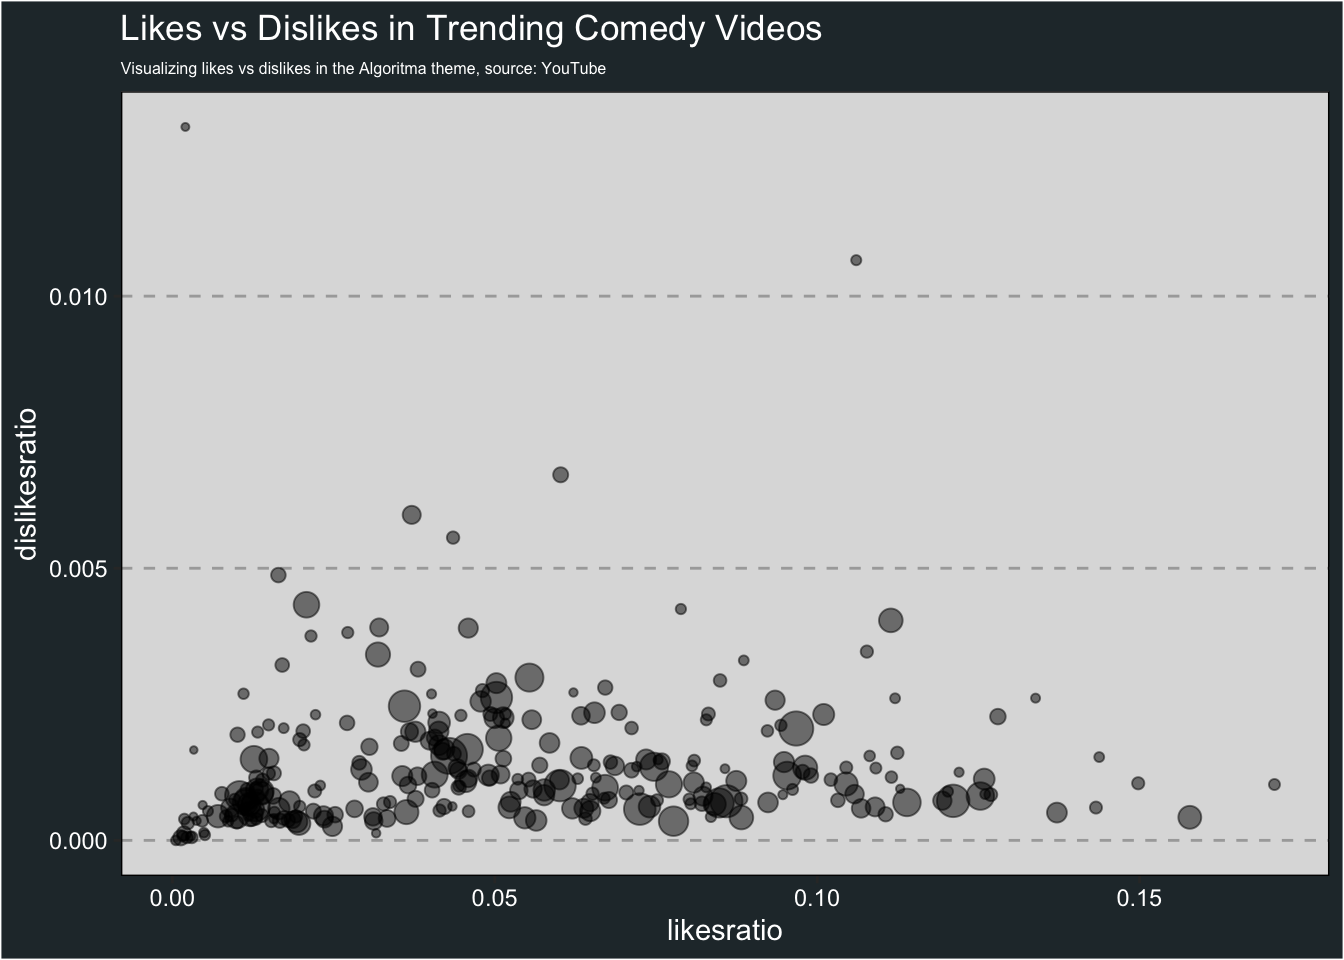
\includegraphics{unsupervised_files/figure-latex/unnamed-chunk-26-1.pdf}

\begin{Shaded}
\begin{Highlighting}[]
\KeywordTok{plot.PCA}\NormalTok{(loan_pca, }\DataTypeTok{cex=}\FloatTok{0.6}\NormalTok{, }\DataTypeTok{choix =} \KeywordTok{c}\NormalTok{(}\StringTok{"var"}\NormalTok{))}
\end{Highlighting}
\end{Shaded}

\includegraphics{unsupervised_files/figure-latex/unnamed-chunk-26-2.pdf}

With your Variables factor map plotted (second plot), let's use the
\texttt{dimdesc()} function to help us understand the variables and the
categories that are the most characteristic according to each dimension
obtained in the PCA process. Notice that I'm looking at the quantitative
variables ``best describe'' the first and second dimensions, and that
the function has automatically sorted the values by descending order.

If you use \texttt{summary(loan\_pca)} you can confirm these correlation
as well. The variables factor map we got above is merely a plot of these
variables using their correlations to Dim 1 and Dim 2 as x and y axis.

Try swapping \texttt{quanti} for \texttt{quali} and you'll get the
qualitative variables. Alternatively, use \texttt{summary()} to inspect
these figures and compare them to the plot you obtain above.

\begin{Shaded}
\begin{Highlighting}[]
\NormalTok{a <-}\StringTok{ }\KeywordTok{dimdesc}\NormalTok{(loan_pca)}
\KeywordTok{as.data.frame}\NormalTok{(a[[}\DecValTok{1}\NormalTok{]]}\OperatorTok{$}\NormalTok{quanti)}
\end{Highlighting}
\end{Shaded}

\begin{verbatim}
##              correlation
## log_inc       0.88500740
## annual_inc    0.87000929
## installment   0.60032845
## revol_bal     0.55896033
## inq_last_12m  0.20578749
## verified      0.18483538
## int_rate      0.13145046
## delinq_2yrs   0.05946769
## grdCtoA      -0.09983199
## dti          -0.21468727
##                                                                                                                                                                        p.value
## log_inc      0.000000000000000000000000000000000000000000000000000000000000000000000000000000000000000000000000000000000000000000000000000000000000000000000000000000000000000
## annual_inc   0.000000000000000000000000000000000000000000000000000000000000000000000000000000000000000000000000000000000000000000000000000000000000000000000000000000000000000
## installment  0.000000000000000000000000000000000000000000000000000000000000000000000000000000000000000000000000000000000000000000000000000000000000000000000000000000005262153
## revol_bal    0.000000000000000000000000000000000000000000000000000000000000000000000000000000000000000000000000000000000000000000000000000000014129656050651152686817218399256
## inq_last_12m 0.000000000000000242578998762364627758465947494467400246983792211005748207242049829801544547080993652343750000000000000000000000000000000000000000000000000000000
## verified     0.000000000000200304148995065031292968143663560712084857270975923881906055612489581108093261718750000000000000000000000000000000000000000000000000000000000000000
## int_rate     0.000000195418368222459672372173897399172393107846801285631954669952392578125000000000000000000000000000000000000000000000000000000000000000000000000000000000000
## delinq_2yrs  0.018977966591853096672837253322541073430329561233520507812500000000000000000000000000000000000000000000000000000000000000000000000000000000000000000000000000000
## grdCtoA      0.000079905835911483412111258606280728145065950229763984680175781250000000000000000000000000000000000000000000000000000000000000000000000000000000000000000000000
## dti          0.000000000000000011111504367670145347770623171498667510491184287602615954337892389958142302930355072021484375000000000000000000000000000000000000000000000000000
\end{verbatim}

Visualizing the correlation between each variables and our PC 2:

\begin{Shaded}
\begin{Highlighting}[]
\NormalTok{a <-}\StringTok{ }\KeywordTok{dimdesc}\NormalTok{(loan_pca)}
\NormalTok{a <-}\StringTok{ }\KeywordTok{as.data.frame}\NormalTok{(a[[}\DecValTok{2}\NormalTok{]]}\OperatorTok{$}\NormalTok{quanti)}
\NormalTok{a <-}\StringTok{ }\KeywordTok{cbind}\NormalTok{(}\KeywordTok{rownames}\NormalTok{(a), a)}
\KeywordTok{plot}\NormalTok{(}\KeywordTok{as.factor}\NormalTok{(a[,}\DecValTok{1}\NormalTok{]), a[,}\DecValTok{2}\NormalTok{])}
\end{Highlighting}
\end{Shaded}

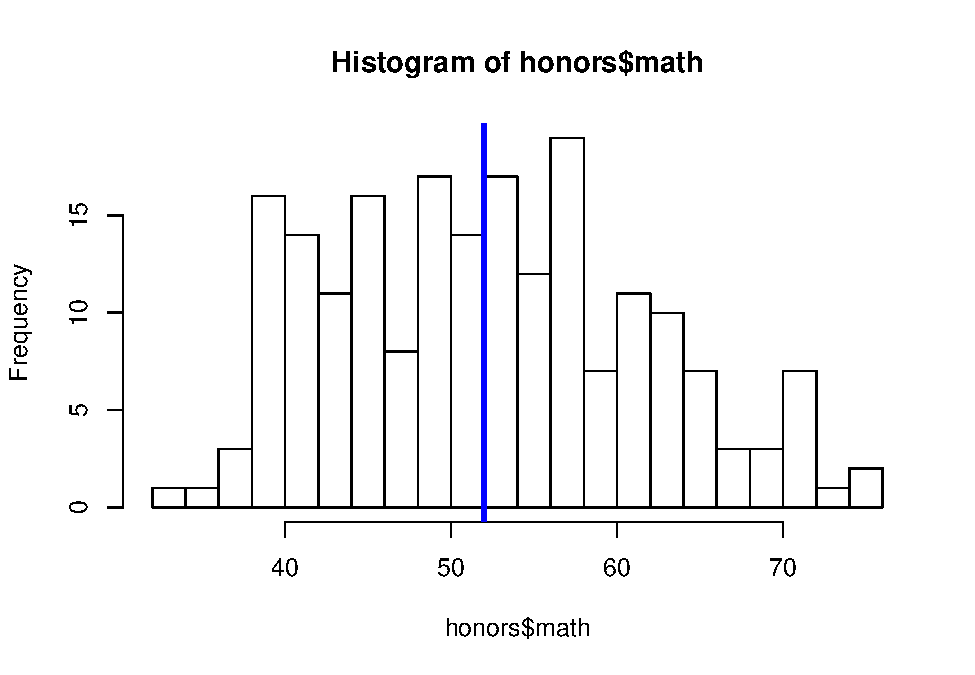
\includegraphics{unsupervised_files/figure-latex/unnamed-chunk-28-1.pdf}

Finally, using \texttt{loan\_pca\$eig}, how many principal components do
you need to retain more than 75\% of the variation in our data? Consider
the tradeoff between dimensionality reduction and the advantages it
offer as we look at yet another area of application for PCA:
classification!

\begin{Shaded}
\begin{Highlighting}[]
\NormalTok{loan_pca}\OperatorTok{$}\NormalTok{eig}
\end{Highlighting}
\end{Shaded}

\begin{verbatim}
##         eigenvalue percentage of variance cumulative percentage of variance
## comp 1   2.3663705              23.663705                          23.66370
## comp 2   2.0160600              20.160600                          43.82431
## comp 3   1.1862316              11.862316                          55.68662
## comp 4   1.0181086              10.181086                          65.86771
## comp 5   0.9205087               9.205087                          75.07279
## comp 6   0.8797229               8.797229                          83.87002
## comp 7   0.7052375               7.052375                          90.92240
## comp 8   0.4934798               4.934798                          95.85720
## comp 9   0.2516231               2.516231                          98.37343
## comp 10  0.1626573               1.626573                         100.00000
\end{verbatim}

We've spent a lot of time understanding that principal components are
just new ``dimensions'' (think ``variables'' if they are more intuitive)
that give us the most value in explaining the variation in our dataset.
This also makes PCA a handy tool to visualize and understand how a
combination of our original explanatory variables (or two combinations)
can sufficiently explain the variation between categories - these are
potentially handy tools for classification cases with high-dimension
datasets!

In the following graph, we see that PC1 and PC2 combined can do a pretty
decent job at classifying the \texttt{grade} of our loan, but not too
well on \texttt{purpose} or \texttt{verification\_status} for example:

\begin{Shaded}
\begin{Highlighting}[]
\CommentTok{# plotellipses(loan_pca, keepvar="quali.sup")}
\NormalTok{loan_pca <-}\StringTok{ }\KeywordTok{PCA}\NormalTok{(loan[,}\KeywordTok{c}\NormalTok{(}\DecValTok{2}\OperatorTok{:}\DecValTok{11}\NormalTok{,}\DecValTok{14}\OperatorTok{:}\DecValTok{16}\NormalTok{)], }\DataTypeTok{quali.sup =} \KeywordTok{c}\NormalTok{(}\DecValTok{1}\NormalTok{,}\DecValTok{6}\NormalTok{,}\DecValTok{7}\NormalTok{), }\DataTypeTok{graph=}\NormalTok{F)}
\KeywordTok{plotellipses}\NormalTok{(loan_pca, }\DataTypeTok{keepvar=}\KeywordTok{c}\NormalTok{(}\DecValTok{1}\NormalTok{,}\DecValTok{6}\NormalTok{,}\DecValTok{7}\NormalTok{))}
\end{Highlighting}
\end{Shaded}

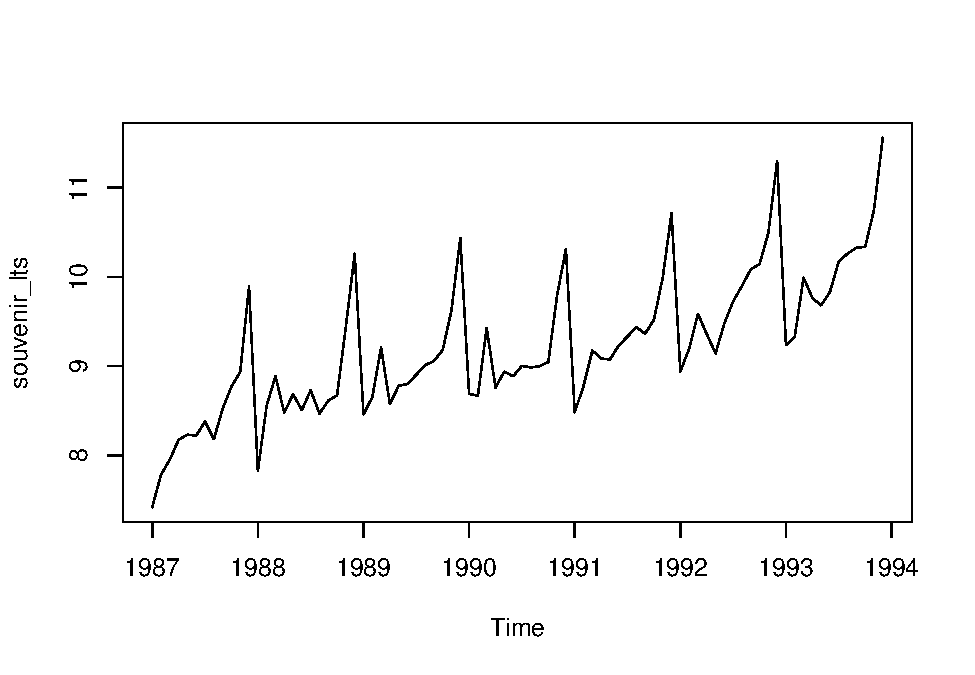
\includegraphics{unsupervised_files/figure-latex/unnamed-chunk-30-1.pdf}

As we move into the next section, let's summarize:\\
- Eigenvectors are just the linear combinations of the original
variables (in the simple or rotated factor space); they described how
variables ``contribute'' to each factor axis\\
- Think of PCA as as way to construct new dimensions (like x and y axes)
that point to the directions of maximal variance (in the original
variable space), as expressed by the eigenvalue\\
- The eigenvalue associated with each principal component also tells you
how much variation in the data set it explains\\
- Data should be normalized before performing PCA. PCA is sensitive to
scaling of data as higher variance data will drive the principal
component.

\hypertarget{practical-application-eigenfaces}{%
\subsection{Practical Application:
Eigenfaces}\label{practical-application-eigenfaces}}

When we develop facial recognition system, we're usually operating in a
very high dimensional space - think, 1024 dimensions (read the
Motivation section at the beginning of this coursebook). Numerous
empirical studies shown that very problematic issues arise out of this
dimensionality especially when our training sample is not sufficiently
large. Remember from a few weeks back we've learned about the Euclidean
distance? It turns out that when Euclidean distance is applied on a
high-dimensional dataset, ``there {[}exist{]} little distance in the
distance between pairs of samples''\footnote{\href{https://en.wikipedia.org/wiki/Curse_of_dimensionality\#Distance_functions}{Wikipedia,
  Curse of Dimensionality - Distance Functions}}." Another undesired
effect of high dimensionality concerns the k-NN nearest neighbor
algorithm we learned about in the Classification 1 workshop, \footnote{\href{http://www.jmlr.org/papers/volume11/radovanovic10a/radovanovic10a.pdf}{Radovanovic,
  Hubs in Space: Popular Nearest Neighbors in high-dimensional data}}
and yet another concerns anomaly detection. The phenomenon of undesired
effect arising out of working with data in high-dimensional spaces
(where they don't occur in low-dimensional settings of everyday
experience) was affectionately called ``the curse of dimensionality''.

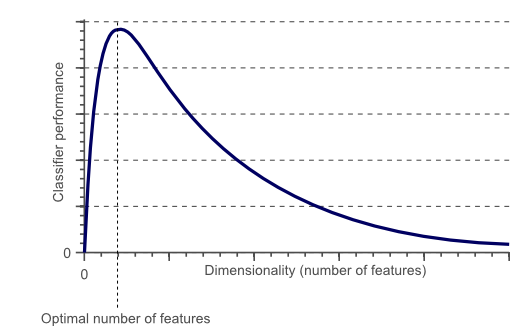
\includegraphics{assets/curseofdim.png}

For images with 1024-dimensions (32 x 32), PCA becomes highly useful as
we look to reduce the number of dimensions in our feature space by
calculating the eigenvectors of the covariance matrix from the original
1024-dimensional data, and then projecting each feature vector onto the
largest eigenvectors. When using only the \textbf{first four
eigenvectors} on the Cambridge face dataset\footnote{\href{http://www.jmlr.org/papers/volume11/radovanovic10a/radovanovic10a.pdf}{Radovanovic,
  Hubs in Space: Popular Nearest Neighbors in high-dimensional data}}:

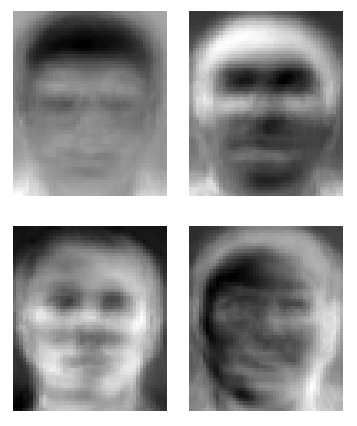
\includegraphics{assets/eigenfaces.png}

Each of the 1024-dimensional feature vector when projected onto the N
largest eigenvectors can hence be represented as a linear combination of
these eigenfaces. We can then have our classifer ``learn'' the
coefficients (beta values) of these linear combinations and predict the
identity of the person. Remember: what we've learned about eigenvectors
still apply: the first PC represents the largest variance in the data,
and the second PC try and capture the most amount of ``error'' from the
first component, and so on. Collectively, the first 4 PCs capture the
most amount of variation / information of a face. If we build a
classifier using only the first 30 eigenvectors, that is a pretty
substantial reduction in dimensionality (from 1024).

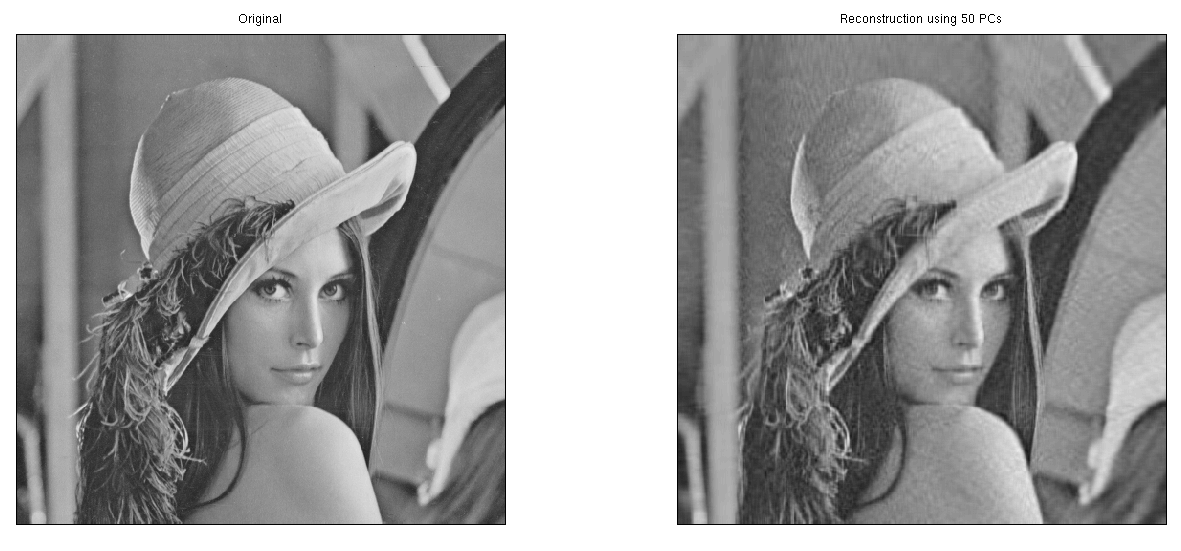
\includegraphics{assets/lenna.png}

In the following example, I'll demonstrate how PCA is used in the field
of image processing by reconstructing a 32x32 image using only the first
4 principal components. The reconstruction of our data was done using
the \texttt{reconst()} function:

\begin{Shaded}
\begin{Highlighting}[]
\KeywordTok{load}\NormalTok{(}\StringTok{"data_input/face.rda"}\NormalTok{)}
\NormalTok{face_pca <-}\StringTok{ }\KeywordTok{PCA}\NormalTok{(faceData,  }\DataTypeTok{graph =}\NormalTok{ F)}
\NormalTok{face_recon <-}\StringTok{ }\KeywordTok{reconst}\NormalTok{(face_pca, }\DataTypeTok{ncp=}\DecValTok{4}\NormalTok{)}
\end{Highlighting}
\end{Shaded}

Taking a look at the eigenvalues will show us that the first 4 will
explain \textasciitilde{}85\% of the variances in our data:

\begin{Shaded}
\begin{Highlighting}[]
\KeywordTok{head}\NormalTok{(face_pca}\OperatorTok{$}\NormalTok{eig)}
\end{Highlighting}
\end{Shaded}

\begin{verbatim}
##        eigenvalue percentage of variance cumulative percentage of variance
## comp 1 12.6194690              39.435841                          39.43584
## comp 2  7.3922489              23.100778                          62.53662
## comp 3  4.7536745              14.855233                          77.39185
## comp 4  2.2909120               7.159100                          84.55095
## comp 5  1.2400024               3.875008                          88.42596
## comp 6  0.7862118               2.456912                          90.88287
\end{verbatim}

So the first principal component (PC1) explains the most variance, the
second explains the next. The variance that each explains is measured by
its eigenvalue, which is scaled in terms of the number of variables
worth of variance. So PC1 in that respect, explains as much variance as
12.62 original variables does. This also mean that the eigenvalues would
sum up to the total number of variables:

\begin{Shaded}
\begin{Highlighting}[]
\KeywordTok{sum}\NormalTok{(face_pca}\OperatorTok{$}\NormalTok{eig[,}\DecValTok{1}\NormalTok{])}
\end{Highlighting}
\end{Shaded}

\begin{verbatim}
## [1] 32
\end{verbatim}

I'm using the \texttt{image()} function from base R to create a grid of
colored (in our case, gray-scale) rectangles with color corresponding to
the values in a given matrix:

\begin{Shaded}
\begin{Highlighting}[]
\NormalTok{showMatrix <-}\StringTok{ }\ControlFlowTok{function}\NormalTok{(x, title)\{}
  \KeywordTok{image}\NormalTok{(}\KeywordTok{t}\NormalTok{(x[}\KeywordTok{nrow}\NormalTok{(x)}\OperatorTok{:}\DecValTok{1}\NormalTok{,]), }
        \DataTypeTok{xaxt =} \StringTok{'n'}\NormalTok{, }\DataTypeTok{yaxt =} \StringTok{'n'}\NormalTok{, }
        \DataTypeTok{col =} \KeywordTok{gray}\NormalTok{((}\DecValTok{0}\OperatorTok{:}\DecValTok{32}\NormalTok{)}\OperatorTok{/}\DecValTok{32}\NormalTok{),}
        \DataTypeTok{main =}\NormalTok{ title, }
        \DataTypeTok{font.main=}\DecValTok{4}\NormalTok{, }
        \DataTypeTok{cex.main=}\FloatTok{0.5}
\NormalTok{        )}
\NormalTok{  \}}
\end{Highlighting}
\end{Shaded}

And here we'll plot the original image as well as the one reconstructed
from 4 principal components:

\begin{Shaded}
\begin{Highlighting}[]
\KeywordTok{par}\NormalTok{(}\DataTypeTok{mfrow=}\KeywordTok{c}\NormalTok{(}\DecValTok{1}\NormalTok{,}\DecValTok{2}\NormalTok{), }\DataTypeTok{mar=}\KeywordTok{c}\NormalTok{(}\FloatTok{0.5}\NormalTok{,}\FloatTok{0.5}\NormalTok{,}\FloatTok{1.5}\NormalTok{,}\FloatTok{0.5}\NormalTok{))}
\KeywordTok{showMatrix}\NormalTok{(faceData, }\DataTypeTok{title =} \StringTok{'Original Image'}\NormalTok{)}
\KeywordTok{showMatrix}\NormalTok{(face_recon, }\DataTypeTok{title =} \StringTok{'Reconstructed w/ 4 dimensions'}\NormalTok{)}
\end{Highlighting}
\end{Shaded}

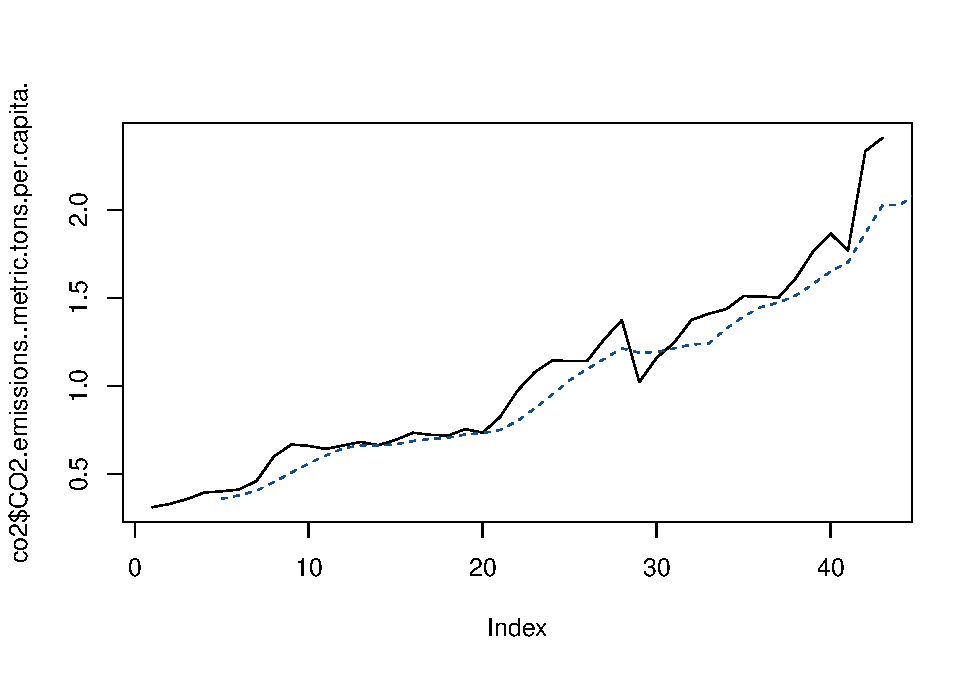
\includegraphics{unsupervised_files/figure-latex/unnamed-chunk-35-1.pdf}

If you did not skip the earlier optional section describing the matrix
algebra behind PCA, you can also create your own reconstruction function
manually:

\begin{Shaded}
\begin{Highlighting}[]
\NormalTok{face_pca_m <-}\StringTok{ }\KeywordTok{prcomp}\NormalTok{(faceData, }\DataTypeTok{center =}\NormalTok{ T, }\DataTypeTok{scale=}\NormalTok{T)}
\NormalTok{prcomp.recon <-}\StringTok{ }\ControlFlowTok{function}\NormalTok{(pca, }\DataTypeTok{pcs=}\OtherTok{NULL}\NormalTok{)\{}
  \ControlFlowTok{if}\NormalTok{(}\KeywordTok{is.null}\NormalTok{(pcs)) pcs <-}\StringTok{ }\KeywordTok{seq}\NormalTok{(pca}\OperatorTok{$}\NormalTok{sdev)}
\NormalTok{  recon <-}\StringTok{ }\KeywordTok{as.matrix}\NormalTok{(pca}\OperatorTok{$}\NormalTok{x[,pcs]) }\OperatorTok\StringTok{ }\KeywordTok{t}\NormalTok{(}\KeywordTok{as.matrix}\NormalTok{(pca}\OperatorTok{$}\NormalTok{rotation[,pcs]))}
  \ControlFlowTok{if}\NormalTok{(pca}\OperatorTok{$}\NormalTok{scale[}\DecValTok{1}\NormalTok{] }\OperatorTok{!=}\StringTok{ }\OtherTok{FALSE}\NormalTok{)\{}
\NormalTok{    recon <-}\StringTok{ }\KeywordTok{scale}\NormalTok{(recon , }\DataTypeTok{center=}\OtherTok{FALSE}\NormalTok{, }\DataTypeTok{scale=}\DecValTok{1}\OperatorTok{/}\NormalTok{pca}\OperatorTok{$}\NormalTok{scale)}
\NormalTok{  \}}
  \ControlFlowTok{if}\NormalTok{(pca}\OperatorTok{$}\NormalTok{center[}\DecValTok{1}\NormalTok{] }\OperatorTok{!=}\StringTok{ }\OtherTok{FALSE}\NormalTok{)\{}
\NormalTok{    recon <-}\StringTok{ }\KeywordTok{scale}\NormalTok{(recon , }\DataTypeTok{center=}\OperatorTok{-}\NormalTok{pca}\OperatorTok{$}\NormalTok{center, }\DataTypeTok{scale=}\OtherTok{FALSE}\NormalTok{)}
\NormalTok{  \}}
\NormalTok{  recon}
\NormalTok{\}}
\end{Highlighting}
\end{Shaded}

Using the manual function we created above, let's compare the 4 images
reconstructed with varying degree of dimensionality:

\begin{Shaded}
\begin{Highlighting}[]
\NormalTok{con_manual3 <-}\StringTok{ }\KeywordTok{prcomp.recon}\NormalTok{(face_pca_m, }\DataTypeTok{pcs=}\DecValTok{1}\OperatorTok{:}\DecValTok{3}\NormalTok{)}
\NormalTok{con_manual10 <-}\StringTok{ }\KeywordTok{prcomp.recon}\NormalTok{(face_pca_m, }\DataTypeTok{pcs=}\DecValTok{1}\OperatorTok{:}\DecValTok{10}\NormalTok{)}
\NormalTok{con_manual15 <-}\StringTok{ }\KeywordTok{prcomp.recon}\NormalTok{(face_pca_m, }\DataTypeTok{pcs=}\DecValTok{1}\OperatorTok{:}\DecValTok{15}\NormalTok{)}

\KeywordTok{par}\NormalTok{(}\DataTypeTok{mfrow=}\KeywordTok{c}\NormalTok{(}\DecValTok{2}\NormalTok{,}\DecValTok{2}\NormalTok{), }\DataTypeTok{mar=}\KeywordTok{c}\NormalTok{(}\FloatTok{0.5}\NormalTok{,}\FloatTok{0.5}\NormalTok{,}\FloatTok{1.5}\NormalTok{,}\FloatTok{0.5}\NormalTok{))}
\KeywordTok{showMatrix}\NormalTok{(faceData, }\DataTypeTok{title =} \StringTok{'Original Image'}\NormalTok{)}
\KeywordTok{showMatrix}\NormalTok{(con_manual3, }\DataTypeTok{title =} \StringTok{'Reconstructed: 3 dimensions'}\NormalTok{)}
\KeywordTok{showMatrix}\NormalTok{(con_manual10, }\DataTypeTok{title =} \StringTok{'Reconstructed: 7 dimensions'}\NormalTok{)}
\KeywordTok{showMatrix}\NormalTok{(con_manual15, }\DataTypeTok{title =} \StringTok{'Reconstructed: 15 dimensions'}\NormalTok{)}
\end{Highlighting}
\end{Shaded}

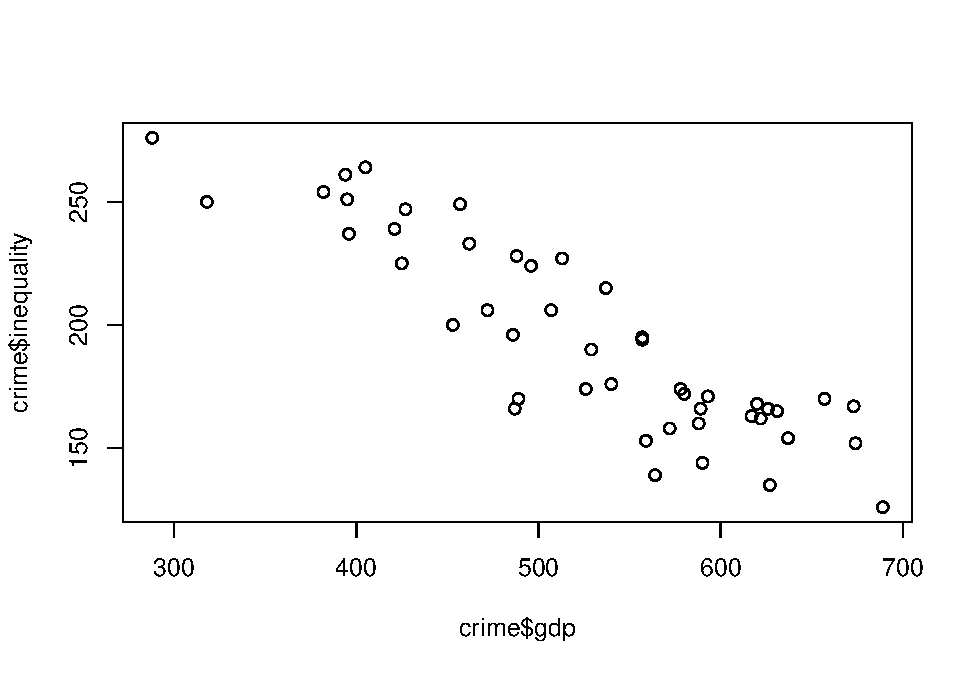
\includegraphics{unsupervised_files/figure-latex/unnamed-chunk-37-1.pdf}

\hypertarget{pca-for-anomaly-detection}{%
\subsubsection{PCA for Anomaly
Detection}\label{pca-for-anomaly-detection}}

We've learned that PCA is used in the area of image compression and also
in more general unsupervised tasks as they are very effective at
revealing the inner structure of (the variance of) our data. There exist
however, many other uses of PCA - one example is in anomaly detection.
When applied as an anomaly detection algorithm, each new observation is
projected on the eigenvectors together with a normalized reconstruction
error. The normalized error error is used as the anomaly score - the
higher the error, the more anomalous the instance is.

PCA thrives where classification algorithms come short in this respect
because very often when dealing with fraudulent transactions, we don't
have enough examples of fraud to train on, but have many examples of
good transactions. In fact, in many cases we also do not know a case of
fraud beforehand, only after-the-fact.

The PCA-Based Anomaly Detection module solves the problem by analyzing
available features to determine what constitutes a ``normal'' class, and
applying distance metrics to identify cases that represent anomalies.
This let you train a model using existing imbalanced data\footnote{\href{https://docs.microsoft.com/en-us/azure/machine-learning/studio-module-reference/pca-based-anomaly-detection}{Microsoft
  Azure, PCA-Based Anomaly Detection}}.

\hypertarget{k-means-clustering}{%
\section{K-means Clustering}\label{k-means-clustering}}

Clustering refers to the practice of finding meaningful ways to group
data (or create subgroups) within a dataset - and the resulting groups
are usually called clusters. The objective is to have a number of
partitions where the observations that fall into each partition are
similar to others in that group, while the partitions are distinctive
from one another.

K-means is a centroid-based clustering algorithm that follows a simple
procedure of classifying a given dataset into a pre-determined number of
clusters, denoted as ``k''. This procedure is essentially a series of
interations where we:\\
1. Find cluster centers\\
2. Compute distances between each point to each cluster centers\\
3. Assign / re-assign cluster membership

A few technicality: Instead of saying ``cluster centers'', we'll call
them ``centroids''; Also, in the first iteration of the above procedure,
because there are clusters in our feature space, we can't yet compute
any centroids so in the first ``iteration'' we'll randomly assign our
centroids. It turns out, with enough iteration, that the procedure can
usually converge at a reasonably well solution, giving us very
reasonable k centroids (remember: we define k, just as in the k-NN
algorithm we learned) that we can use for clustering task.

Run the following code in your console to see an animation that
illustrate the k-means algorithm in action:

\begin{Shaded}
\begin{Highlighting}[]
\KeywordTok{library}\NormalTok{(animation)}
\CommentTok{## set larger 'interval' if the speed is too fast}
\KeywordTok{ani.options}\NormalTok{(}\DataTypeTok{interval =} \DecValTok{1}\NormalTok{)}
\KeywordTok{par}\NormalTok{(}\DataTypeTok{mar =} \KeywordTok{c}\NormalTok{(}\DecValTok{3}\NormalTok{, }\DecValTok{3}\NormalTok{, }\DecValTok{1}\NormalTok{, }\FloatTok{1.5}\NormalTok{), }\DataTypeTok{mgp =} \KeywordTok{c}\NormalTok{(}\FloatTok{1.5}\NormalTok{, }\FloatTok{0.5}\NormalTok{, }\DecValTok{0}\NormalTok{))}
\KeywordTok{kmeans.ani}\NormalTok{()}
\end{Highlighting}
\end{Shaded}

Let's take a look at the image below:
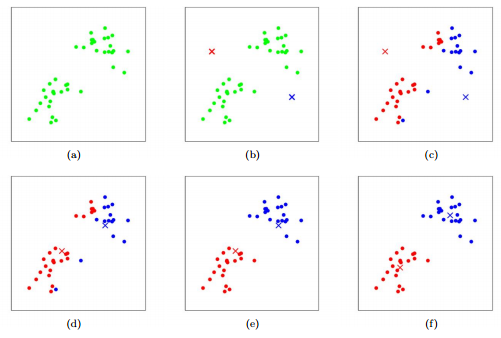
\includegraphics{assets/centroids.png}

If we choose \emph{k} to be 2, these are the steps that a k-means
algorithm take in assigning the original data (green dots) to two
clusters:\\
Step (a): Our data on a two-dimensional space\\
Step (b): Iteration 1 - Randomly initialize our cluster centroids\\
Step (c): Iteration 1 - Assigning cluster membership based on a distance
function\\
Step (d): Iteration 2 - Move cluster centroids to be at the center of
clusters\\
Step (e): Iteration 2 - Re-Assigning cluster membership based on a
distance function\\
Step (f): Iteration 3 \ldots{}

We'll get into the mathematical details a bit later; For now, let's take
a look at how we can use R's \texttt{kmeans()} function to solve a
clustering problem in the absence of a target predictor.

\hypertarget{cluster-based-whisky-recommendation}{%
\subsection{Cluster-based Whisky
Recommendation}\label{cluster-based-whisky-recommendation}}

The data we'll be reading in is from Dr.Wisehart (University of
St.~Andrews), and comprise of 86 distilleries that produce malt
whiskies. Each of the whiskies were scored between 0-4 under 12
different taste categories including \texttt{Body}, \texttt{Sweetness},
\texttt{Smoky}, \texttt{Medicinal}, \texttt{Tobacco}, \texttt{Honey},
\texttt{Nutty}, \texttt{Floral} etc. The original motivation also notes
that ``by using correlation data it may be possible to provide whisky
recommendations based upon an individual's particular
preferences''{[}{]}.

\begin{Shaded}
\begin{Highlighting}[]
\CommentTok{# Read data in}
\NormalTok{whiskies <-}\StringTok{ }\KeywordTok{read.csv}\NormalTok{(}\StringTok{"data_input/whiskies.txt"}\NormalTok{)}
\CommentTok{# Distillery column is the name of each whisky}
\KeywordTok{rownames}\NormalTok{(whiskies) <-}\StringTok{ }\NormalTok{whiskies[,}\StringTok{"Distillery"}\NormalTok{]}

\CommentTok{# remove RowID, Postcode, Latitude and Longitude}
\NormalTok{whiskies <-}\StringTok{ }\NormalTok{whiskies[,}\DecValTok{3}\OperatorTok{:}\DecValTok{14}\NormalTok{]}
\end{Highlighting}
\end{Shaded}

We'll perform scaling, just as we did in the PCA analyses earlier. With
this dataset - scaling is rather arbitary and optional because all
measurments assume the same range (0 to 4), but with most data this
won't be the case. Recall that the \texttt{kmeans} procedure compute a
distance (typically Euclidean distance) and as we've learned in the k-NN
section of this Specialization, failing to scale may cause our model to
perform adequately with the algorithm favoring variables on higher
scales.

\begin{Shaded}
\begin{Highlighting}[]
\NormalTok{whi_z <-}\StringTok{ }\KeywordTok{scale}\NormalTok{(whiskies)}
\end{Highlighting}
\end{Shaded}

We will have to set a seed for reproducibility because in the first
iteration, our centroids are randomly picked on the feature space - thus
each time we run the \texttt{kmeans()} we are bound to get a slightly
different result. Given the objective of \textbf{minimizing the
within-cluster sum of squared} the k-means algorithm is guaranteed to
converge but is not guaranteed to a global optima - a point I'll
illustrate later through some code experiment.

\begin{Shaded}
\begin{Highlighting}[]
\KeywordTok{set.seed}\NormalTok{(}\DecValTok{100}\NormalTok{)}
\CommentTok{# k-means with 4 clusters}
\NormalTok{whi_km <-}\StringTok{ }\KeywordTok{kmeans}\NormalTok{(whi_z, }\DecValTok{4}\NormalTok{)}
\NormalTok{whi_km}\OperatorTok{$}\NormalTok{centers}
\end{Highlighting}
\end{Shaded}

\begin{verbatim}
##         Body    Sweetness       Smoky  Medicinal   Tobacco      Honey
## 1  0.4940232  0.004767928  0.09583381 -0.3143508 -0.360623  0.6790443
## 2  1.2685075 -1.102344865  1.98597755  2.4781900  1.190056 -1.1652785
## 3 -0.6689511  0.218421273 -0.49746877 -0.2596258 -0.360623 -0.3170533
## 4 -0.2541181  0.059440164 -0.04039276  0.1213648  2.740735 -0.2862087
##        Spicy      Winey      Nutty      Malty      Fruity      Floral
## 1  0.3730788  0.7501678  0.3645842  0.3609734  0.14040770 -0.05919838
## 2  0.3074849 -0.6451223 -0.1096666 -0.6792715 -0.70862009 -1.69315362
## 3 -0.4554755 -0.5675370 -0.2457723 -0.2714167  0.08479886  0.38436842
## 4  0.3605847  0.2036135 -0.3631969  0.5791521 -0.38787626  0.15866232
\end{verbatim}

\begin{Shaded}
\begin{Highlighting}[]
\NormalTok{whi_km}\OperatorTok{$}\NormalTok{iter}
\end{Highlighting}
\end{Shaded}

\begin{verbatim}
## [1] 3
\end{verbatim}

When we use \texttt{\$iter}, we see that k-means take only 3 iterations
to converge, stopping at the third iteration: it already identified 4
sufficiently distinct clusters and further iteration wouldn't improve it
any further. The objective has been satisfied. The original algorithm by
Lloyd uses this as the objective (minimizing the within-cluster sum of
squares):

\(\sum\limits^k_{i=1}\sum\limits_{x_j \in S_i} (x_j - \mu_i)^2\)

Where \(\mu_i\) is the mean of all the points in cluster \(S_i\)

Now let's make this whole idea a lot more concrete by working with some
simulated data in code.

\hypertarget{dive-deeper-understanding-k-means}{%
\subsubsection{Dive Deeper: Understanding
k-means}\label{dive-deeper-understanding-k-means}}

In the following experiment, we'll observe how the initialization may
not converge to the global optima by simulating some data and changing
the seed number iteratively. Here's the code to generate some random
data:

\begin{Shaded}
\begin{Highlighting}[]
\KeywordTok{set.seed}\NormalTok{(}\DecValTok{100}\NormalTok{)}
\NormalTok{x1 <-}\StringTok{ }\KeywordTok{runif}\NormalTok{(}\DecValTok{100}\NormalTok{, }\DecValTok{1}\NormalTok{, }\DecValTok{2}\NormalTok{)}
\NormalTok{y1 <-}\StringTok{ }\KeywordTok{runif}\NormalTok{(}\DecValTok{100}\NormalTok{, }\DecValTok{1}\NormalTok{, }\DecValTok{2}\NormalTok{)}
\NormalTok{x2 <-}\StringTok{ }\KeywordTok{runif}\NormalTok{(}\DecValTok{100}\NormalTok{, }\FloatTok{0.4}\NormalTok{, }\FloatTok{1.5}\NormalTok{)}
\NormalTok{y2 <-}\StringTok{ }\KeywordTok{runif}\NormalTok{(}\DecValTok{100}\NormalTok{, }\FloatTok{0.4}\NormalTok{, }\FloatTok{1.5}\NormalTok{)}
\NormalTok{a <-}\StringTok{ }\KeywordTok{rbind}\NormalTok{(}\KeywordTok{data.frame}\NormalTok{(}\DataTypeTok{x=}\NormalTok{x1,}\DataTypeTok{y=}\NormalTok{y1), }\KeywordTok{data.frame}\NormalTok{(}\DataTypeTok{x=}\NormalTok{x2,}\DataTypeTok{y=}\NormalTok{y2))}
\KeywordTok{head}\NormalTok{(a)}
\end{Highlighting}
\end{Shaded}

\begin{verbatim}
##          x        y
## 1 1.307766 1.327415
## 2 1.257673 1.389479
## 3 1.552322 1.041053
## 4 1.056383 1.361397
## 5 1.468549 1.570978
## 6 1.483771 1.684880
\end{verbatim}

Plotting \texttt{a\$x} and \texttt{a\$y} will yield the following:

\begin{Shaded}
\begin{Highlighting}[]
\KeywordTok{plot}\NormalTok{(a}\OperatorTok{$}\NormalTok{x, a}\OperatorTok{$}\NormalTok{y, }\DataTypeTok{xlim=}\KeywordTok{c}\NormalTok{(}\DecValTok{0}\NormalTok{, }\FloatTok{2.5}\NormalTok{), }\DataTypeTok{ylim=}\KeywordTok{c}\NormalTok{(}\DecValTok{0}\NormalTok{,}\FloatTok{2.5}\NormalTok{), }\DataTypeTok{pch=}\DecValTok{19}\NormalTok{, }\DataTypeTok{cex=}\FloatTok{0.4}\NormalTok{)}
\end{Highlighting}
\end{Shaded}

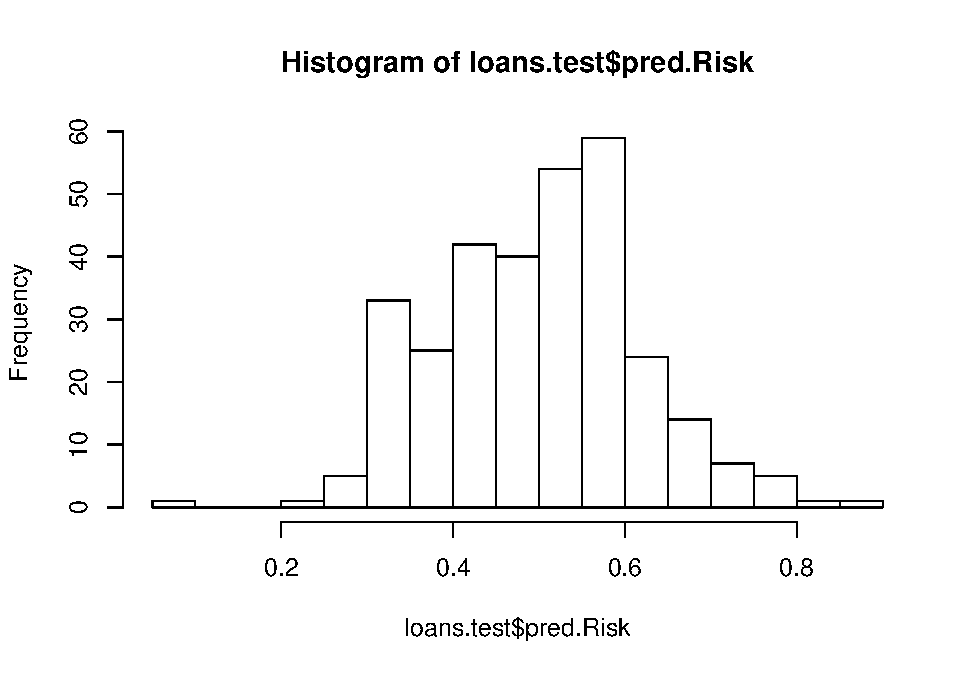
\includegraphics{unsupervised_files/figure-latex/unnamed-chunk-43-1.pdf}

By eye-balling the data, one may make a reasonable argument that there
can be three clusters. I'm going to run \texttt{kmeans()} on the
simulated data, specifying 3 so the k-means algorithm would use 3 number
of clusters. Later, you may want to change the seed from 50 to 100 so
you can get a visual idea of how the initialization of our centroids
will lead to a rather different outcome:

\begin{Shaded}
\begin{Highlighting}[]
\KeywordTok{set.seed}\NormalTok{(}\DecValTok{50}\NormalTok{)}
\NormalTok{a_k <-}\StringTok{ }\KeywordTok{kmeans}\NormalTok{(a[,}\DecValTok{1}\OperatorTok{:}\DecValTok{2}\NormalTok{], }\DecValTok{3}\NormalTok{)}
\NormalTok{a}\OperatorTok{$}\NormalTok{clus <-}\StringTok{ }\NormalTok{a_k}\OperatorTok{$}\NormalTok{cluster}
\NormalTok{a_k}\OperatorTok{$}\NormalTok{centers}
\end{Highlighting}
\end{Shaded}

\begin{verbatim}
##           x         y
## 1 0.8087252 0.9008249
## 2 1.6184781 1.7396137
## 3 1.3536168 1.1725641
\end{verbatim}

With the kmeans model \texttt{a\_k}, we'll now plot our clusters
(square) and map the color of our points to the assigned clusters from
our \texttt{a\_k\$cluster}:

\begin{Shaded}
\begin{Highlighting}[]
\KeywordTok{plot}\NormalTok{(a}\OperatorTok{$}\NormalTok{x, a}\OperatorTok{$}\NormalTok{y, }\DataTypeTok{xlim=}\KeywordTok{c}\NormalTok{(}\DecValTok{0}\NormalTok{, }\FloatTok{2.5}\NormalTok{), }\DataTypeTok{ylim=}\KeywordTok{c}\NormalTok{(}\DecValTok{0}\NormalTok{,}\FloatTok{2.5}\NormalTok{), }\DataTypeTok{pch=}\DecValTok{19}\NormalTok{, }\DataTypeTok{cex=}\FloatTok{0.4}\NormalTok{, }\DataTypeTok{col=}\NormalTok{a}\OperatorTok{$}\NormalTok{clus)}
\KeywordTok{points}\NormalTok{(a_k}\OperatorTok{$}\NormalTok{centers, }\DataTypeTok{col=}\DecValTok{1}\OperatorTok{:}\DecValTok{3}\NormalTok{, }\DataTypeTok{pch=}\DecValTok{15}\NormalTok{, }\DataTypeTok{cex=}\FloatTok{1.5}\NormalTok{)}
\end{Highlighting}
\end{Shaded}

\includegraphics{unsupervised_files/figure-latex/unnamed-chunk-45-1.pdf}

Try changing the seed from 50 to a different number and observe how the
initialization would lead us to a model with different centroids, and
consequently different within-cluster sum of squares as well as the sum
of within-cluster of squares.

According to our original model, our within-cluster sum of squares can
be computed by subtracting each point's x and y coordinates to the
centroid's x and y coordinates, then taking the sum of the squared
values. This, we learn in previous workshops, is the Euclidean's
distance:

\begin{Shaded}
\begin{Highlighting}[]
\CommentTok{# sum of square distance for cluster 1}
\NormalTok{ssd1 <-}\StringTok{ }\KeywordTok{sum}\NormalTok{((a[a}\OperatorTok{$}\NormalTok{clus}\OperatorTok{==}\DecValTok{1}\NormalTok{, }\DecValTok{1}\NormalTok{] }\OperatorTok{-}\StringTok{ }\NormalTok{a_k}\OperatorTok{$}\NormalTok{centers[}\DecValTok{1}\NormalTok{,}\DecValTok{1}\NormalTok{])}\OperatorTok{^}\DecValTok{2} \OperatorTok{+}\StringTok{ }\NormalTok{((a[a}\OperatorTok{$}\NormalTok{clus}\OperatorTok{==}\DecValTok{1}\NormalTok{, }\DecValTok{2}\NormalTok{] }\OperatorTok{-}\StringTok{ }\NormalTok{a_k}\OperatorTok{$}\NormalTok{centers[}\DecValTok{1}\NormalTok{,}\DecValTok{2}\NormalTok{])}\OperatorTok{^}\DecValTok{2}\NormalTok{))}

\CommentTok{# sum of square distance for cluster 2 }
\NormalTok{ssd2 <-}\StringTok{ }\KeywordTok{sum}\NormalTok{((a[a}\OperatorTok{$}\NormalTok{clus}\OperatorTok{==}\DecValTok{2}\NormalTok{, }\DecValTok{1}\NormalTok{] }\OperatorTok{-}\StringTok{ }\NormalTok{a_k}\OperatorTok{$}\NormalTok{centers[}\DecValTok{2}\NormalTok{,}\DecValTok{1}\NormalTok{])}\OperatorTok{^}\DecValTok{2} \OperatorTok{+}\StringTok{ }\NormalTok{((a[a}\OperatorTok{$}\NormalTok{clus}\OperatorTok{==}\DecValTok{2}\NormalTok{, }\DecValTok{2}\NormalTok{] }\OperatorTok{-}\StringTok{ }\NormalTok{a_k}\OperatorTok{$}\NormalTok{centers[}\DecValTok{2}\NormalTok{,}\DecValTok{2}\NormalTok{])}\OperatorTok{^}\DecValTok{2}\NormalTok{))}

\CommentTok{# sum of square distance for cluster 3}
\NormalTok{ssd3 <-}\StringTok{ }\KeywordTok{sum}\NormalTok{((a[a}\OperatorTok{$}\NormalTok{clus}\OperatorTok{==}\DecValTok{3}\NormalTok{, }\DecValTok{1}\NormalTok{] }\OperatorTok{-}\StringTok{ }\NormalTok{a_k}\OperatorTok{$}\NormalTok{centers[}\DecValTok{3}\NormalTok{,}\DecValTok{1}\NormalTok{])}\OperatorTok{^}\DecValTok{2} \OperatorTok{+}\StringTok{ }\NormalTok{((a[a}\OperatorTok{$}\NormalTok{clus}\OperatorTok{==}\DecValTok{3}\NormalTok{, }\DecValTok{2}\NormalTok{] }\OperatorTok{-}\StringTok{ }\NormalTok{a_k}\OperatorTok{$}\NormalTok{centers[}\DecValTok{3}\NormalTok{,}\DecValTok{2}\NormalTok{])}\OperatorTok{^}\DecValTok{2}\NormalTok{))}

\KeywordTok{c}\NormalTok{(ssd1, ssd2, ssd3)}
\end{Highlighting}
\end{Shaded}

\begin{verbatim}
## [1] 8.466600 4.776666 6.846074
\end{verbatim}

\begin{Shaded}
\begin{Highlighting}[]
\KeywordTok{sum}\NormalTok{(ssd1, ssd2, ssd3)}
\end{Highlighting}
\end{Shaded}

\begin{verbatim}
## [1] 20.08934
\end{verbatim}

The \texttt{kmeans} model we obtained (we named it \texttt{a\_k}) also
has methods that output these two figures:

\begin{Shaded}
\begin{Highlighting}[]
\NormalTok{a_k}\OperatorTok{$}\NormalTok{withinss}
\end{Highlighting}
\end{Shaded}

\begin{verbatim}
## [1] 8.466600 4.776666 6.846074
\end{verbatim}

\begin{Shaded}
\begin{Highlighting}[]
\NormalTok{a_k}\OperatorTok{$}\NormalTok{tot.withinss}
\end{Highlighting}
\end{Shaded}

\begin{verbatim}
## [1] 20.08934
\end{verbatim}

If we print \texttt{a\_k} we will see ``between SS / total SS =
67.8\%'', this can serve as another indicator for the goodness of fit.
When we compute the sum of squared distances of each point to the global
sample mean, we get the total sum of squares. That's also computed for
us by \texttt{kmeans()} and accessible via \texttt{\$totss}:

\begin{Shaded}
\begin{Highlighting}[]
\KeywordTok{sum}\NormalTok{((a}\OperatorTok{$}\NormalTok{x }\OperatorTok{-}\StringTok{ }\KeywordTok{mean}\NormalTok{(a}\OperatorTok{$}\NormalTok{x))}\OperatorTok{^}\DecValTok{2} \OperatorTok{+}\StringTok{ }\NormalTok{(a}\OperatorTok{$}\NormalTok{y }\OperatorTok{-}\StringTok{ }\KeywordTok{mean}\NormalTok{(a}\OperatorTok{$}\NormalTok{y))}\OperatorTok{^}\DecValTok{2}\NormalTok{)}
\end{Highlighting}
\end{Shaded}

\begin{verbatim}
## [1] 62.46317
\end{verbatim}

\begin{Shaded}
\begin{Highlighting}[]
\NormalTok{a_k}\OperatorTok{$}\NormalTok{totss}
\end{Highlighting}
\end{Shaded}

\begin{verbatim}
## [1] 62.46317
\end{verbatim}

However, when we choose to compute one per cluster (we have 3 clusters)
instead of using the global sample mean - and then find the sum of
squared distances of these three means to the global mean, we get the
between sum of squares (\texttt{\$betweenss}). When we do this, we also
multiply the squared distance of each mean to the global mean by the
number of data points it represents:

\begin{Shaded}
\begin{Highlighting}[]
\KeywordTok{sum}\NormalTok{((a_k}\OperatorTok{$}\NormalTok{centers[}\DecValTok{1}\NormalTok{,}\DecValTok{1}\NormalTok{] }\OperatorTok{-}\StringTok{ }\KeywordTok{mean}\NormalTok{(a}\OperatorTok{$}\NormalTok{x))}\OperatorTok{^}\DecValTok{2} \OperatorTok{+}\StringTok{ }\NormalTok{(a_k}\OperatorTok{$}\NormalTok{centers[}\DecValTok{1}\NormalTok{,}\DecValTok{2}\NormalTok{] }\OperatorTok{-}\StringTok{ }\KeywordTok{mean}\NormalTok{(a}\OperatorTok{$}\NormalTok{y))}\OperatorTok{^}\DecValTok{2}\NormalTok{)}\OperatorTok{*}\NormalTok{a_k}\OperatorTok{$}\NormalTok{size[}\DecValTok{1}\NormalTok{]}\OperatorTok{+}
\KeywordTok{sum}\NormalTok{((a_k}\OperatorTok{$}\NormalTok{centers[}\DecValTok{2}\NormalTok{,}\DecValTok{1}\NormalTok{] }\OperatorTok{-}\StringTok{ }\KeywordTok{mean}\NormalTok{(a}\OperatorTok{$}\NormalTok{x))}\OperatorTok{^}\DecValTok{2} \OperatorTok{+}\StringTok{ }\NormalTok{(a_k}\OperatorTok{$}\NormalTok{centers[}\DecValTok{2}\NormalTok{,}\DecValTok{2}\NormalTok{] }\OperatorTok{-}\StringTok{ }\KeywordTok{mean}\NormalTok{(a}\OperatorTok{$}\NormalTok{y))}\OperatorTok{^}\DecValTok{2}\NormalTok{)}\OperatorTok{*}\NormalTok{a_k}\OperatorTok{$}\NormalTok{size[}\DecValTok{2}\NormalTok{]}\OperatorTok{+}
\KeywordTok{sum}\NormalTok{((a_k}\OperatorTok{$}\NormalTok{centers[}\DecValTok{3}\NormalTok{,}\DecValTok{1}\NormalTok{] }\OperatorTok{-}\StringTok{ }\KeywordTok{mean}\NormalTok{(a}\OperatorTok{$}\NormalTok{x))}\OperatorTok{^}\DecValTok{2} \OperatorTok{+}\StringTok{ }\NormalTok{(a_k}\OperatorTok{$}\NormalTok{centers[}\DecValTok{3}\NormalTok{,}\DecValTok{2}\NormalTok{] }\OperatorTok{-}\StringTok{ }\KeywordTok{mean}\NormalTok{(a}\OperatorTok{$}\NormalTok{y))}\OperatorTok{^}\DecValTok{2}\NormalTok{)}\OperatorTok{*}\NormalTok{a_k}\OperatorTok{$}\NormalTok{size[}\DecValTok{3}\NormalTok{]}
\end{Highlighting}
\end{Shaded}

\begin{verbatim}
## [1] 42.37383
\end{verbatim}

\begin{Shaded}
\begin{Highlighting}[]
\NormalTok{a_k}\OperatorTok{$}\NormalTok{betweenss}
\end{Highlighting}
\end{Shaded}

\begin{verbatim}
## [1] 42.37383
\end{verbatim}

Taking the ratio of \texttt{betweenss} and \texttt{totss} we get 67.8\%
which is the same as what the output of \texttt{a\_k} gives us when we
print \texttt{a\_k}:

\begin{Shaded}
\begin{Highlighting}[]
\NormalTok{a_k}\OperatorTok{$}\NormalTok{betweenss}\OperatorTok{/}\NormalTok{a_k}\OperatorTok{$}\NormalTok{totss}\OperatorTok{*}\DecValTok{100}
\end{Highlighting}
\end{Shaded}

\begin{verbatim}
## [1] 67.8381
\end{verbatim}

We said earlier that this can be taken as a goodness of the clustering
model our k-means has found. It can be thought of as the decomposition
of deviance in deviance ``between'' and deviance ``within'' - we want a
clustering model that has strong properties of internal cohesion and
maximal external separation and so the between sum of squares and total
sum of squares ratio as close to 1 as possible indicates a good fit.

Let's repeat the same experiment; this time we'll specify for 4 centers
instead:

\begin{Shaded}
\begin{Highlighting}[]
\KeywordTok{set.seed}\NormalTok{(}\DecValTok{50}\NormalTok{)}
\NormalTok{a_k2 <-}\StringTok{ }\KeywordTok{kmeans}\NormalTok{(a[,}\DecValTok{1}\OperatorTok{:}\DecValTok{2}\NormalTok{], }\DecValTok{4}\NormalTok{)}
\NormalTok{a}\OperatorTok{$}\NormalTok{clus2 <-}\StringTok{ }\NormalTok{a_k2}\OperatorTok{$}\NormalTok{cluster}
\KeywordTok{plot}\NormalTok{(a}\OperatorTok{$}\NormalTok{x, a}\OperatorTok{$}\NormalTok{y, }\DataTypeTok{xlim=}\KeywordTok{c}\NormalTok{(}\DecValTok{0}\NormalTok{, }\FloatTok{2.5}\NormalTok{), }\DataTypeTok{ylim=}\KeywordTok{c}\NormalTok{(}\DecValTok{0}\NormalTok{,}\FloatTok{2.5}\NormalTok{), }\DataTypeTok{pch=}\DecValTok{19}\NormalTok{, }\DataTypeTok{cex=}\FloatTok{0.4}\NormalTok{, }\DataTypeTok{col=}\NormalTok{a}\OperatorTok{$}\NormalTok{clus2)}
\KeywordTok{points}\NormalTok{(a_k2}\OperatorTok{$}\NormalTok{centers, }\DataTypeTok{col=}\DecValTok{1}\OperatorTok{:}\DecValTok{4}\NormalTok{, }\DataTypeTok{pch=}\DecValTok{15}\NormalTok{, }\DataTypeTok{cex=}\FloatTok{1.5}\NormalTok{)}
\end{Highlighting}
\end{Shaded}

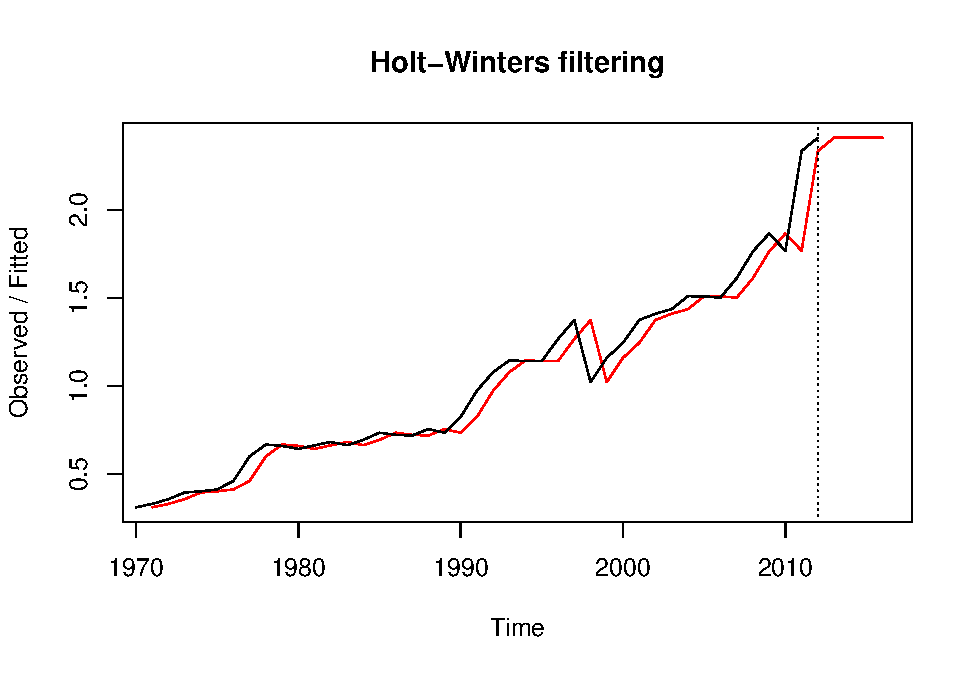
\includegraphics{unsupervised_files/figure-latex/unnamed-chunk-51-1.pdf}

This is a better ``fit'' as it has stronger ``between-cluster''
separation (pay special attention to the black and blue clusters). The
BSS/TSS ratio gives us a confirmation of that as well:

\begin{Shaded}
\begin{Highlighting}[]
\NormalTok{a_k2}\OperatorTok{$}\NormalTok{betweenss}\OperatorTok{/}\NormalTok{a_k2}\OperatorTok{$}\NormalTok{totss}\OperatorTok{*}\DecValTok{100}
\end{Highlighting}
\end{Shaded}

\begin{verbatim}
## [1] 75.50799
\end{verbatim}

Note that however, we can arbitarily improve the ``goodness'' of model
by just increasing \emph{k}, so the quality as I've mentioned above is
purely mathematical and may not reflect the user's requirement. Often
times, as with the case of whiskies clustering, we want to consider
external information when picking a good value of k.

Run the function below and observe that our within sum of squares
decrease as we naively increase the number of clusters - what we're
looking for is a point where diminishing returns start to kick in (an
elbow) and we start to lose substantial gains: we'll use that point as
the number of clusters (\emph{k}) for our kmeans model:

\begin{Shaded}
\begin{Highlighting}[]
\NormalTok{wss <-}\StringTok{ }\ControlFlowTok{function}\NormalTok{(data, }\DataTypeTok{maxCluster =} \DecValTok{9}\NormalTok{) \{}
    \CommentTok{# Initialize within sum of squares}
\NormalTok{    SSw <-}\StringTok{ }\NormalTok{(}\KeywordTok{nrow}\NormalTok{(data) }\OperatorTok{-}\StringTok{ }\DecValTok{1}\NormalTok{) }\OperatorTok{*}\StringTok{ }\KeywordTok{sum}\NormalTok{(}\KeywordTok{apply}\NormalTok{(data, }\DecValTok{2}\NormalTok{, var))}
\NormalTok{    SSw <-}\StringTok{ }\KeywordTok{vector}\NormalTok{()}
    \ControlFlowTok{for}\NormalTok{ (i }\ControlFlowTok{in} \DecValTok{2}\OperatorTok{:}\NormalTok{maxCluster) \{}
\NormalTok{        SSw[i] <-}\StringTok{ }\KeywordTok{sum}\NormalTok{(}\KeywordTok{kmeans}\NormalTok{(data, }\DataTypeTok{centers =}\NormalTok{ i)}\OperatorTok{$}\NormalTok{withinss)}
\NormalTok{    \}}
    \KeywordTok{plot}\NormalTok{(}\DecValTok{1}\OperatorTok{:}\NormalTok{maxCluster, SSw, }\DataTypeTok{type =} \StringTok{"o"}\NormalTok{, }\DataTypeTok{xlab =} \StringTok{"Number of Clusters"}\NormalTok{, }\DataTypeTok{ylab =} \StringTok{"Within groups sum of squares"}\NormalTok{, }\DataTypeTok{pch=}\DecValTok{19}\NormalTok{)}
\NormalTok{\}}
\KeywordTok{wss}\NormalTok{(whi_z)}
\end{Highlighting}
\end{Shaded}

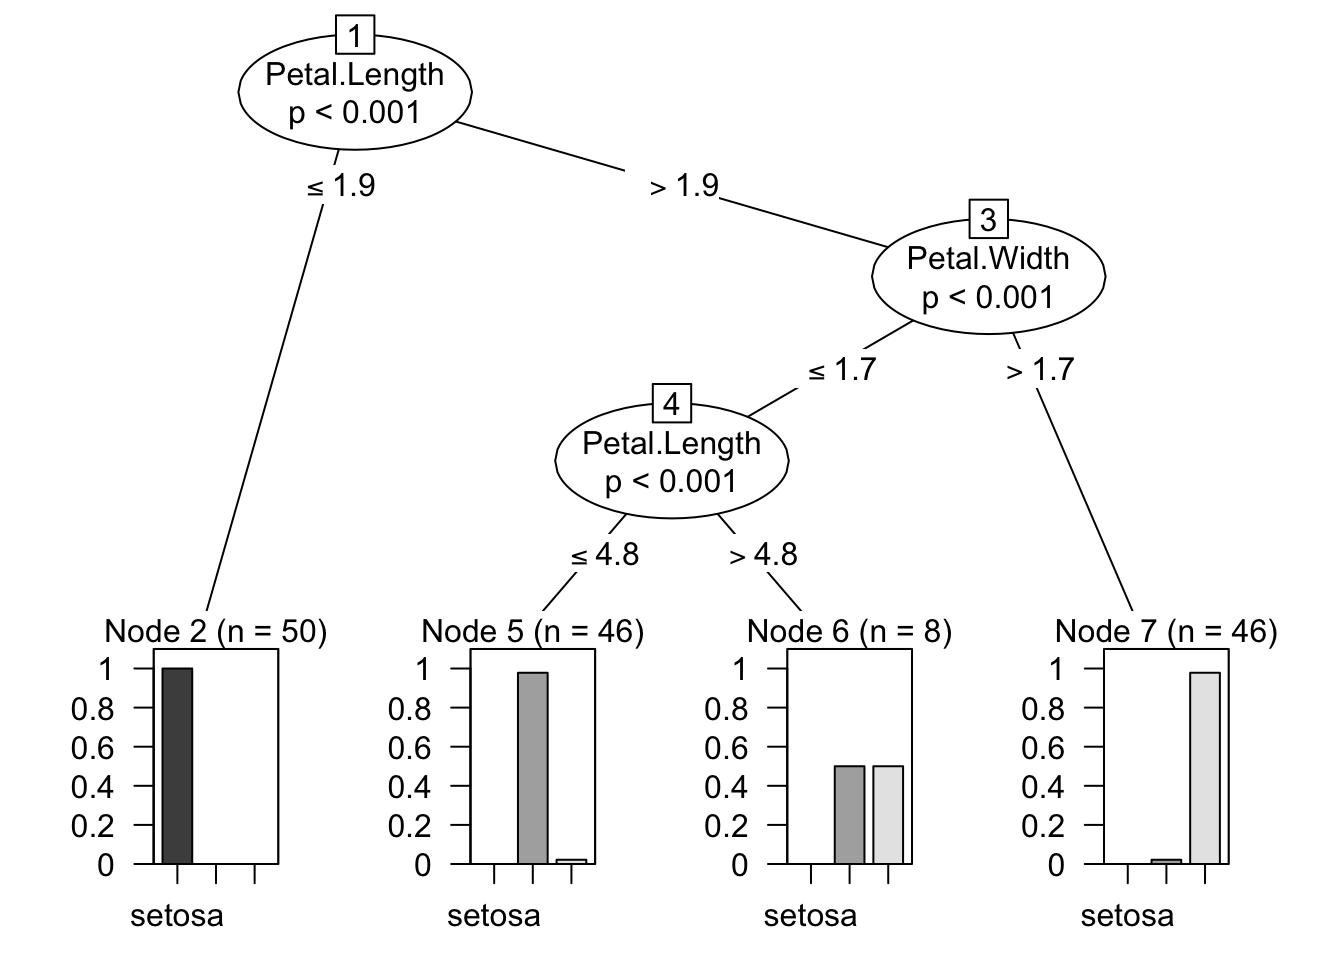
\includegraphics{unsupervised_files/figure-latex/unnamed-chunk-53-1.pdf}

Choosing k=4, we'll create our kmeans model (\texttt{whi\_km}) and we
will append the cluster to our original data in a variable named
\texttt{clust}:

\begin{Shaded}
\begin{Highlighting}[]
\NormalTok{whi_km <-}\StringTok{ }\KeywordTok{kmeans}\NormalTok{(whi_z, }\DecValTok{4}\NormalTok{)}
\NormalTok{whiskies}\OperatorTok{$}\NormalTok{clust <-}\StringTok{ }\KeywordTok{as.factor}\NormalTok{(whi_km}\OperatorTok{$}\NormalTok{cluster)}
\end{Highlighting}
\end{Shaded}

\textbf{Discussion:} Now assuming a long-time customer of ours reveal
that him (and his spouse) enjoy Laphroig the most, what other whiskies
can we recommend?

\begin{Shaded}
\begin{Highlighting}[]
\NormalTok{whiskies[}\KeywordTok{rownames}\NormalTok{(whiskies) }\OperatorTok{==}\StringTok{ "Laphroig"}\NormalTok{, ]}
\end{Highlighting}
\end{Shaded}

\begin{verbatim}
##          Body Sweetness Smoky Medicinal Tobacco Honey Spicy Winey Nutty Malty
## Laphroig    4         2     4         4       1     0     0     1     1     1
##          Fruity Floral clust
## Laphroig      0      0     3
\end{verbatim}

\hypertarget{combining-pca-with-k-means}{%
\subsection{Combining PCA with
k-means}\label{combining-pca-with-k-means}}

Now that we have learned k-means and PCA, let's use the combination of
both to visualize where our Laphroig whiskey sits in a two-dimensional
space. I'm creating the PCA using the \texttt{FactoMineR} package, and
the points are colored based on the assigned cluster created in previous
steps.

In the resulting plot, observe the cluster memberships on our two
dimensions (PC1 and PC2) - remark on whether the two dimensions have
captured the variations between these 4 distinct groups of whiskies
sufficiently. It is helpful to recall that prior to our PCA, there is no
data reduction yet - k-means was grouping our points with the objective
of getting good internal cohesion and external separation \textbf{on the
original dimensional space!}. The original dimensional space, however,
is 13-dimensional and that is difficult to visualize meaningfully.

We'll label the point ``Laphroig'' on our biplot, and we'll do the full
process from start to finish as an additional practice:

\begin{Shaded}
\begin{Highlighting}[]
\KeywordTok{library}\NormalTok{(FactoMineR)}
\KeywordTok{set.seed}\NormalTok{(}\DecValTok{100}\NormalTok{)}

\NormalTok{whiskies <-}\StringTok{ }\KeywordTok{read.csv}\NormalTok{(}\StringTok{"data_input/whiskies.txt"}\NormalTok{)}
\KeywordTok{rownames}\NormalTok{(whiskies) <-}\StringTok{ }\NormalTok{whiskies}\OperatorTok{$}\NormalTok{Distillery}
\NormalTok{whiskies <-}\StringTok{ }\NormalTok{whiskies[,}\DecValTok{3}\OperatorTok{:}\DecValTok{14}\NormalTok{]}
\NormalTok{whiskies_z <-}\StringTok{ }\KeywordTok{data.frame}\NormalTok{(}\KeywordTok{scale}\NormalTok{(whiskies))}

\NormalTok{whi_km <-}\StringTok{ }\KeywordTok{kmeans}\NormalTok{(whiskies_z, }\DecValTok{4}\NormalTok{)}
\CommentTok{# creating the 13th column}
\NormalTok{whiskies_z}\OperatorTok{$}\NormalTok{clust <-}\StringTok{ }\KeywordTok{as.factor}\NormalTok{(whi_km}\OperatorTok{$}\NormalTok{cluster)}

\CommentTok{# creates biplots}
\NormalTok{whis.pca <-}\StringTok{ }\KeywordTok{PCA}\NormalTok{(whiskies_z, }\DataTypeTok{quali.sup=}\DecValTok{13}\NormalTok{, }\DataTypeTok{graph =}\NormalTok{ F)}
\CommentTok{# plot(whis.pca, choix=c("ind"), label="none", col.ind=whiskies_z$clust)}
\KeywordTok{plot}\NormalTok{(whis.pca, }\DataTypeTok{choix=}\KeywordTok{c}\NormalTok{(}\StringTok{"ind"}\NormalTok{), }\DataTypeTok{select=}\StringTok{"Laphroig"}\NormalTok{, }\DataTypeTok{habillage=}\DecValTok{13}\NormalTok{)}
\end{Highlighting}
\end{Shaded}

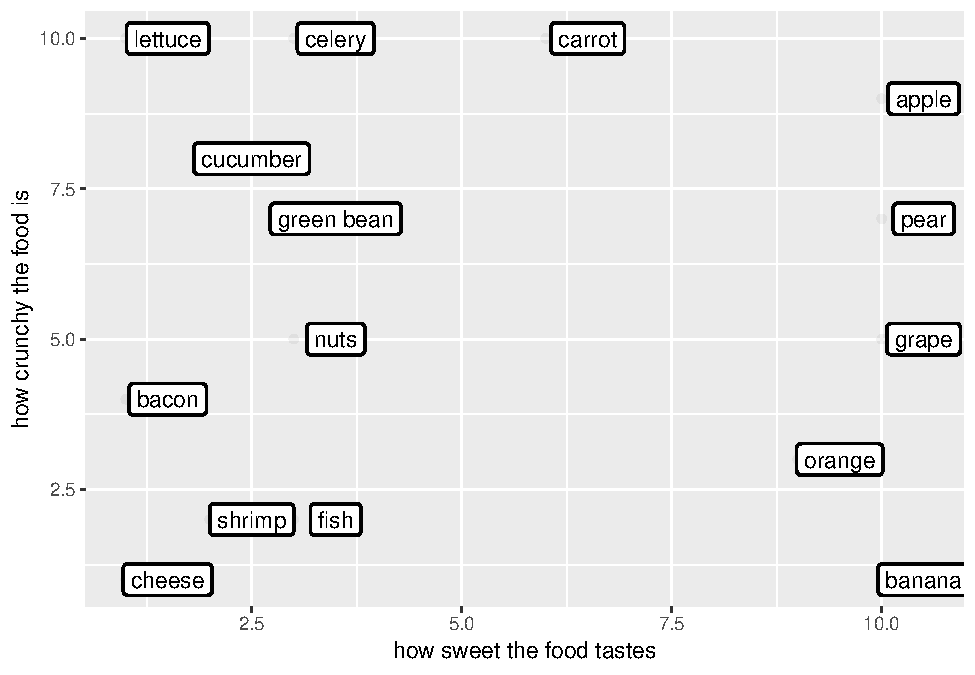
\includegraphics{unsupervised_files/figure-latex/unnamed-chunk-56-1.pdf}

Seeing that Laphroig has a very high value on PC1, it'd be nice to see
the variables that contribute to it:

\begin{Shaded}
\begin{Highlighting}[]
\KeywordTok{plot}\NormalTok{(whis.pca, }\DataTypeTok{choix=}\StringTok{"varcor"}\NormalTok{, }\DataTypeTok{col.ind=}\NormalTok{whiskies}\OperatorTok{$}\NormalTok{clust)}
\end{Highlighting}
\end{Shaded}

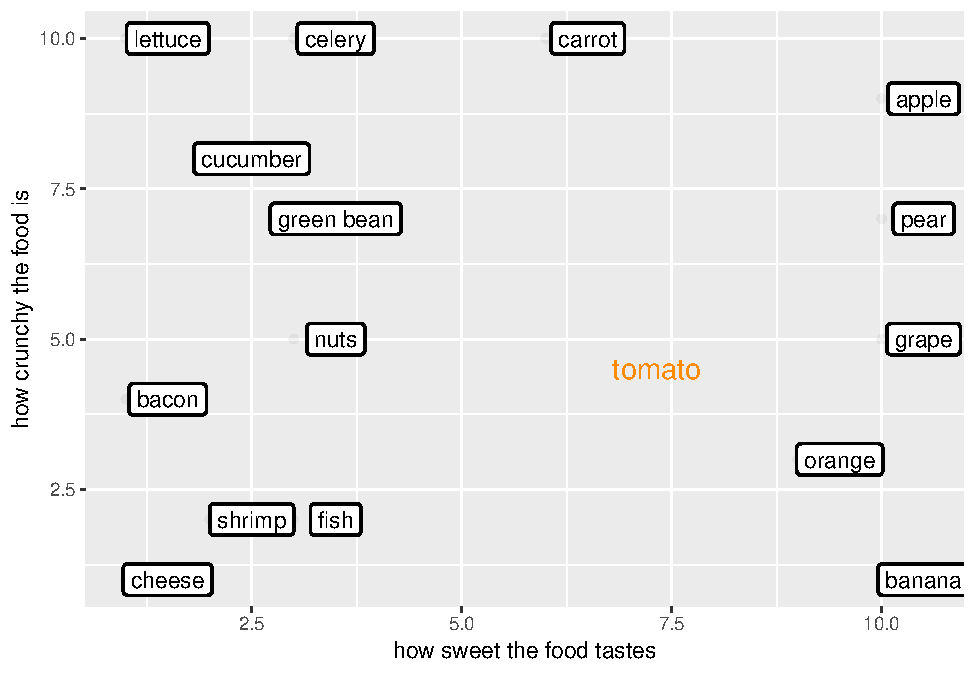
\includegraphics{unsupervised_files/figure-latex/unnamed-chunk-57-1.pdf}

Use the original data as a reference:

\begin{Shaded}
\begin{Highlighting}[]
\NormalTok{whiskies[}\StringTok{"Laphroig"}\NormalTok{, ]}
\end{Highlighting}
\end{Shaded}

\begin{verbatim}
##          Body Sweetness Smoky Medicinal Tobacco Honey Spicy Winey Nutty Malty
## Laphroig    4         2     4         4       1     0     0     1     1     1
##          Fruity Floral
## Laphroig      0      0
\end{verbatim}

\hypertarget{graded-quiz}{%
\section{Graded Quiz}\label{graded-quiz}}

This section of the workshop needs to be completed in the classroom in
order to obtain a score that count towards your final grade.

\hypertarget{learn-by-building}{%
\subsubsection{Learn by building}\label{learn-by-building}}

Using any of the two unsupervised learning algorithms you've learned,
produce a simple R markdown document where you demonstrate an exercise
of either clustering or dimensionality reduction on one of either the
\texttt{wholesale.csv} or the \texttt{nyc} dataset.

Explain your choice of parameters (how you choose \emph{k} for k-means
clustering, or how you choose to retain \emph{n} number of dimensions
for PCA) from the original data. What are some business utility for the
unsupervised model you've developed? The R Markdown document should be
not longer than 4 paragraph, and contain one or two visualization.

\hypertarget{optional-principal-components-by-hand}{%
\subsubsection{{[}Optional{]} Principal Components by
hand}\label{optional-principal-components-by-hand}}

Supposed we create a matrix A, we can compute the eigenvalues and
eigenvectors of this matrix using \texttt{eigen()}:

\begin{Shaded}
\begin{Highlighting}[]
\NormalTok{A <-}\StringTok{ }\KeywordTok{matrix}\NormalTok{(}\KeywordTok{c}\NormalTok{(}\DecValTok{1}\NormalTok{,}\OperatorTok{-}\DecValTok{1}\NormalTok{,}\DecValTok{0}\NormalTok{,}\DecValTok{1}\NormalTok{,}\DecValTok{2}\NormalTok{,}\DecValTok{1}\NormalTok{,}\OperatorTok{-}\DecValTok{2}\NormalTok{,}\DecValTok{1}\NormalTok{,}\OperatorTok{-}\DecValTok{1}\NormalTok{),}\DecValTok{3}\NormalTok{,}\DecValTok{3}\NormalTok{)}
\NormalTok{A}
\end{Highlighting}
\end{Shaded}

\begin{verbatim}
##      [,1] [,2] [,3]
## [1,]    1    1   -2
## [2,]   -1    2    1
## [3,]    0    1   -1
\end{verbatim}

\begin{Shaded}
\begin{Highlighting}[]
\KeywordTok{eigen}\NormalTok{(A)}\OperatorTok{$}\NormalTok{vectors}
\end{Highlighting}
\end{Shaded}

\begin{verbatim}
##           [,1]       [,2]                      [,3]
## [1,] 0.3015113 -0.8017837  0.7071067811865472396704
## [2,] 0.9045340 -0.5345225 -0.0000000000000001922963
## [3,] 0.3015113 -0.2672612  0.7071067811865476837596
\end{verbatim}

Take the eigenvectors multiply the matrix, and notice the direction
don't change (only magnitude change):

\begin{Shaded}
\begin{Highlighting}[]
\NormalTok{A }\OperatorTok\StringTok{ }\KeywordTok{eigen}\NormalTok{(A)}\OperatorTok{$}\NormalTok{vectors}
\end{Highlighting}
\end{Shaded}

\begin{verbatim}
##           [,1]       [,2]                      [,3]
## [1,] 0.6030227 -0.8017837 -0.7071067811865483498934
## [2,] 1.8090681 -0.5345225  0.0000000000000001110223
## [3,] 0.6030227 -0.2672612 -0.7071067811865479058042
\end{verbatim}

Notice that the changes in magnitude is the eigenvalues.

\begin{Shaded}
\begin{Highlighting}[]
\KeywordTok{eigen}\NormalTok{(A)}\OperatorTok{$}\NormalTok{values}
\end{Highlighting}
\end{Shaded}

\begin{verbatim}
## [1]  2  1 -1
\end{verbatim}

\begin{Shaded}
\begin{Highlighting}[]
\NormalTok{ev <-}\StringTok{ }\KeywordTok{diag}\NormalTok{(}\KeywordTok{eigen}\NormalTok{(A)}\OperatorTok{$}\NormalTok{values)}
\NormalTok{ev}
\end{Highlighting}
\end{Shaded}

\begin{verbatim}
##      [,1] [,2] [,3]
## [1,]    2    0    0
## [2,]    0    1    0
## [3,]    0    0   -1
\end{verbatim}

\begin{Shaded}
\begin{Highlighting}[]
\KeywordTok{round}\NormalTok{(}\KeywordTok{eigen}\NormalTok{(A)}\OperatorTok{$}\NormalTok{vectors }\OperatorTok\StringTok{ }\NormalTok{ev }\OperatorTok\StringTok{  }\KeywordTok{solve}\NormalTok{(}\KeywordTok{eigen}\NormalTok{(A)}\OperatorTok{$}\NormalTok{vectors),}\DecValTok{1}\NormalTok{)}
\end{Highlighting}
\end{Shaded}

\begin{verbatim}
##      [,1] [,2] [,3]
## [1,]    1    1   -2
## [2,]   -1    2    1
## [3,]    0    1   -1
\end{verbatim}

Using it on the property dataset:

\begin{Shaded}
\begin{Highlighting}[]
\CommentTok{# transpose eigenvectors}
\NormalTok{ppt_cor <-}\StringTok{ }\KeywordTok{cor}\NormalTok{(ppt_z)}
\KeywordTok{round}\NormalTok{(ppt_cor, }\DecValTok{2}\NormalTok{)}
\end{Highlighting}
\end{Shaded}

\begin{verbatim}
##                           RESIDENTIAL.UNITS COMMERCIAL.UNITS TOTAL.UNITS
## RESIDENTIAL.UNITS                      1.00             0.01        0.85
## COMMERCIAL.UNITS                       0.01             1.00        0.54
## TOTAL.UNITS                            0.85             0.54        1.00
## LAND.SQUARE.FEET                       0.40             0.05        0.37
## GROSS.SQUARE.FEET                      0.64             0.07        0.57
## YEAR.BUILT                             0.03             0.01        0.03
## TAX.CLASS.AT.TIME.OF.SALE              0.02             0.05        0.05
## SALE.PRICE                             0.19             0.06        0.19
##                           LAND.SQUARE.FEET GROSS.SQUARE.FEET YEAR.BUILT
## RESIDENTIAL.UNITS                     0.40              0.64       0.03
## COMMERCIAL.UNITS                      0.05              0.07       0.01
## TOTAL.UNITS                           0.37              0.57       0.03
## LAND.SQUARE.FEET                      1.00              0.61       0.01
## GROSS.SQUARE.FEET                     0.61              1.00       0.03
## YEAR.BUILT                            0.01              0.03       1.00
## TAX.CLASS.AT.TIME.OF.SALE             0.06              0.12      -0.22
## SALE.PRICE                            0.05              0.42       0.01
##                           TAX.CLASS.AT.TIME.OF.SALE SALE.PRICE
## RESIDENTIAL.UNITS                              0.02       0.19
## COMMERCIAL.UNITS                               0.05       0.06
## TOTAL.UNITS                                    0.05       0.19
## LAND.SQUARE.FEET                               0.06       0.05
## GROSS.SQUARE.FEET                              0.12       0.42
## YEAR.BUILT                                    -0.22       0.01
## TAX.CLASS.AT.TIME.OF.SALE                      1.00       0.12
## SALE.PRICE                                     0.12       1.00
\end{verbatim}

\begin{Shaded}
\begin{Highlighting}[]
\NormalTok{ppt_eig <-}\StringTok{ }\KeywordTok{eigen}\NormalTok{(ppt_cor)}
\NormalTok{ppt_eig}
\end{Highlighting}
\end{Shaded}

\begin{verbatim}
## eigen() decomposition
## $values
## [1] 2.9203596646 1.2410086844 1.1776269162 0.9806130752 0.7726815270
## [6] 0.6769599816 0.2307277113 0.0000224397
## 
## $vectors
##             [,1]         [,2]        [,3]        [,4]        [,5]       [,6]
## [1,] -0.49773999 -0.102976993  0.10643637  0.16614221  0.27800741 -0.4760055
## [2,] -0.18571758 -0.077912824 -0.81405372 -0.14422494 -0.16028117  0.3205801
## [3,] -0.51727853 -0.126040658 -0.34177266  0.06361289  0.14748958 -0.2324165
## [4,] -0.37447474 -0.004956048  0.26695842  0.38007119 -0.39187291  0.5460339
## [5,] -0.50062528  0.067209255  0.27685299 -0.07063571 -0.06044181  0.1661533
## [6,] -0.01634503 -0.651890224  0.13704217 -0.36393906 -0.59032493 -0.2729910
## [7,] -0.08105858  0.695392849 -0.09509469 -0.03840370 -0.57066405 -0.4151237
## [8,] -0.22911167  0.233163802  0.18286979 -0.81497199  0.20954732  0.2098045
##             [,7]           [,8]
## [1,]  0.20622559  0.59692573227
## [2,] -0.08125378  0.37535378768
## [3,]  0.13086663 -0.70907321160
## [4,]  0.43852681 -0.00006376875
## [5,] -0.79495917 -0.00026435602
## [6,]  0.02306944  0.00004369453
## [7,]  0.03675596  0.00206556720
## [8,]  0.32801481 -0.00020590174
\end{verbatim}

Notice the first eigenvalue 2.92 is much larger than the second (1.24)
and so on.. the highest eigenvalues correspond to the first principal
components

\begin{Shaded}
\begin{Highlighting}[]
\KeywordTok{sum}\NormalTok{(ppt_eig}\OperatorTok{$}\NormalTok{values)}
\end{Highlighting}
\end{Shaded}

\begin{verbatim}
## [1] 8
\end{verbatim}

\begin{Shaded}
\begin{Highlighting}[]
\KeywordTok{ncol}\NormalTok{(ppt_z)}
\end{Highlighting}
\end{Shaded}

\begin{verbatim}
## [1] 8
\end{verbatim}

Computing the new dataset:

Transpose eigenvectors and data

\begin{Shaded}
\begin{Highlighting}[]
\CommentTok{# eigvt: 8 x 8}
\NormalTok{eigvt <-}\StringTok{ }\KeywordTok{t}\NormalTok{(ppt_eig}\OperatorTok{$}\NormalTok{vectors)}
\CommentTok{# pptt: 8 x 48243}
\NormalTok{pptt <-}\StringTok{ }\KeywordTok{t}\NormalTok{(ppt_z)}

\CommentTok{# the new dataset}
\NormalTok{ppt_pc <-}\StringTok{ }\NormalTok{eigvt }\OperatorTok\StringTok{ }\NormalTok{pptt}

\CommentTok{# transpose it to reverse the previous transposition}
\NormalTok{ppt_pc <-}\StringTok{ }\KeywordTok{t}\NormalTok{(ppt_pc)}
\KeywordTok{colnames}\NormalTok{(ppt_pc) <-}\StringTok{ }\KeywordTok{c}\NormalTok{(}\StringTok{"PC1"}\NormalTok{, }\StringTok{"PC2"}\NormalTok{, }\StringTok{"PC3"}\NormalTok{, }\StringTok{"PC4"}\NormalTok{, }\StringTok{"PC5"}\NormalTok{, }\StringTok{"PC6"}\NormalTok{, }\StringTok{"PC7"}\NormalTok{, }\StringTok{"PC8"}\NormalTok{)}
\end{Highlighting}
\end{Shaded}

\begin{Shaded}
\begin{Highlighting}[]
\KeywordTok{head}\NormalTok{(ppt_pc)}
\end{Highlighting}
\end{Shaded}

\begin{verbatim}
##             PC1       PC2          PC3        PC4        PC5        PC6
## [1,] -0.3439546 0.4623508  0.085490110 -0.5831322 -0.2469415 -0.2843658
## [2,] -0.5558159 0.3142065 -0.009210573 -0.2761992 -0.2206629 -0.5348078
## [3,] -0.4097472 0.4821670  0.092072222 -0.6836529 -0.1967039 -0.2880773
## [4,] -0.3787778 0.3027941 -0.031048289 -0.2384062 -0.2812611 -0.5036195
## [5,] -1.8539398 0.4876897  0.233870790 -1.2390552  0.3312269 -0.6793536
## [6,] -0.8396252 0.3611049  0.217624467 -0.9377999 -0.2207385 -0.3819289
##            PC7         PC8
## [1,] 0.1732473 0.001816628
## [2,] 0.1639657 0.001901269
## [3,] 0.3033094 0.001805151
## [4,] 0.1647015 0.001933826
## [5,] 0.5779248 0.001574494
## [6,] 0.2718612 0.001706892
\end{verbatim}

\begin{Shaded}
\begin{Highlighting}[]
\KeywordTok{apply}\NormalTok{(ppt_pc,}\DecValTok{2}\NormalTok{, }\DataTypeTok{FUN=}\NormalTok{sd)}
\end{Highlighting}
\end{Shaded}

\begin{verbatim}
##         PC1         PC2         PC3         PC4         PC5         PC6 
## 1.708905985 1.114005693 1.085185199 0.990259095 0.879023053 0.822775778 
##         PC7         PC8 
## 0.480341245 0.004737056
\end{verbatim}

\begin{Shaded}
\begin{Highlighting}[]
\NormalTok{ppt_pcauto <-}\StringTok{ }\KeywordTok{prcomp}\NormalTok{(ppt_z)}
\NormalTok{ppt_pcauto}\OperatorTok{$}\NormalTok{sdev}
\end{Highlighting}
\end{Shaded}

\begin{verbatim}
## [1] 1.708905985 1.114005693 1.085185199 0.990259095 0.879023053 0.822775778
## [7] 0.480341245 0.004737056
\end{verbatim}

\begin{Shaded}
\begin{Highlighting}[]
\KeywordTok{head}\NormalTok{(ppt_pcauto}\OperatorTok{$}\NormalTok{x)}
\end{Highlighting}
\end{Shaded}

\begin{verbatim}
##             PC1        PC2          PC3       PC4        PC5        PC6
## [1,] -0.3439546 -0.4623508  0.085490110 0.5831322 -0.2469415 -0.2843658
## [2,] -0.5558159 -0.3142065 -0.009210573 0.2761992 -0.2206629 -0.5348078
## [3,] -0.4097472 -0.4821670  0.092072222 0.6836529 -0.1967039 -0.2880773
## [4,] -0.3787778 -0.3027941 -0.031048289 0.2384062 -0.2812611 -0.5036195
## [5,] -1.8539398 -0.4876897  0.233870790 1.2390552  0.3312269 -0.6793536
## [6,] -0.8396252 -0.3611049  0.217624467 0.9377999 -0.2207385 -0.3819289
##             PC7          PC8
## [1,] -0.1732473 -0.001816628
## [2,] -0.1639657 -0.001901269
## [3,] -0.3033094 -0.001805151
## [4,] -0.1647015 -0.001933826
## [5,] -0.5779248 -0.001574494
## [6,] -0.2718612 -0.001706892
\end{verbatim}

\hypertarget{annotation}{%
\section{Annotation}\label{annotation}}

\end{document}
